\documentclass[a4paper]{tufte-book}
\usepackage{lmodern}% http://ctan.org/pkg/lm
\newcounter{ccounter}
\newcounter{clatihan}
\newcounter{clisting}
\renewcommand\theccounter{\arabic{ccounter}}
\renewcommand\theclatihan{\arabic{clatihan}}
\renewcommand\theclisting{\arabic{clisting}}
\usepackage{soul,color}
\usepackage{placeins}
\usepackage{algorithmic}
\usepackage{algorithm}
\usepackage{listings}
\usepackage{lstlinebgrd}
\usepackage{graphicx}
\usepackage{makeidx}
\usepackage{mathtools}
\usepackage{bookmark}
\usepackage{xcolor}
\usepackage{mathpazo}
\usepackage{multirow}
\definecolor{codegreen}{rgb}{0,0.6,0}
\definecolor{codegray}{rgb}{0.5,0.5,0.5}
\definecolor{codepurple}{rgb}{0.58,0,0.82}
\definecolor{backcolour}{rgb}{0.95,0.95,0.92}
\definecolor{codehighlight}{rgb}{1,0.65,0.65}
 
\lstdefinestyle{pylist}{
    backgroundcolor=\color{backcolour},   
    commentstyle=\color{codegreen},
    keywordstyle=\color{magenta},
    numberstyle=\tiny\color{codegray},
    stringstyle=\color{codepurple},
    basicstyle=\footnotesize,
    breakatwhitespace=false,         
    breaklines=true,                 
    captionpos=b,                    
    keepspaces=true,                 
    numbers=left,                    
    numbersep=5pt,                  
    showspaces=false,                
    showstringspaces=false,
    showtabs=false,                  
    tabsize=2
}
 
\lstset{style=pylist}

\author{STMIK Mikroskil}
\title{Desain dan Analisis Algoritma}
\publisher{Teknik Informatika -- STMIK Mikroskil}
\newenvironment{myindentpar}[1]%
{
	\begin{list}{}%
  {
  	\setlength{\leftmargin}{#1}}%
    \item[]%
	}
{\end{list}}

\newenvironment{contoh}{
	\refstepcounter{ccounter}
	\begin{myindentpar}{1cm}
	\textbf{\underline{Contoh \arabic{ccounter}}}
}{	
	\end{myindentpar}
}

\newenvironment{latihan}{
	\refstepcounter{clatihan}
	\begin{myindentpar}{1cm}
	\textbf{\underline{Latihan \arabic{clatihan}}}	
}{	
	\end{myindentpar}
}

\newenvironment{konsep}{
	\begin{latihan}
	\small\textbf{(Konsep)}
}{
	\end{latihan}
}

\newenvironment{teori}{
    \begin{myindentpar}{1cm}
    \textbf{\underline{Teori}}
}{
    \end{myindentpar}
}

\newenvironment{pemrograman}{
	\begin{latihan}
	\small\textbf{(Pemrograman)}
}{
	\end{latihan}
}

\newenvironment{proyek}{
	\begin{latihan}
	\small\textbf{(Kelompok)}
}{
	\end{latihan}
}

\newenvironment{listprog}[1]{
	\refstepcounter{clisting}
	\begin{myindentpar}{1cm}
	\textbf{\underline{Listing \arabic{clisting}} {#1}}
	
}{
	\end{myindentpar}
}

\renewcommand{\lstlistingname}{Algoritma}% Listing -> Algoritma
\renewcommand{\lstlistlistingname}{Daftar \lstlistingname s}% List of Listings -> Daftar Algoritma

\makeatletter

\makeatletter

\makeindex
\begin{document}

\maketitle
%\tableofcontents
%\renewcommand{\chaptername}{Modul}
\renewcommand{\figurename}{Gambar}
\floatname{algorithm}{Algoritma}

%\chapter{Pengantar dan Model Matematika Big O}\label{ch:modul1}

\section{Pendahuluan}

\newthought{Algoritma} merupakan sebuah rangkaian proses komputasional yang mengkonversi satu atau beberapa masukan (\textit{input}) menjadi satu set keluaran (\textit{output}) jika memungkinkan. Untuk menyelesaikan permasalahan secara baik menggunakan algoritma, kita memerlukan tahapan analisis dan desain algoritma yang tepat dan benar. Tahapan desain akan menentukan bagaimana merancang algoritma kita sedangkan tahapan analisis akan menentukan seberapa banyak ruang (\textit{space}) dan seberapa lama waktu (\textit{time}) yang dibutuhkan algoritma tersebut. Secara umum langkah-langkah dalam penyelesaian masalah bisa dilihat di Gambar~\ref{fig:TahapanAnalisisDanDesain}.

\begin{figure}
    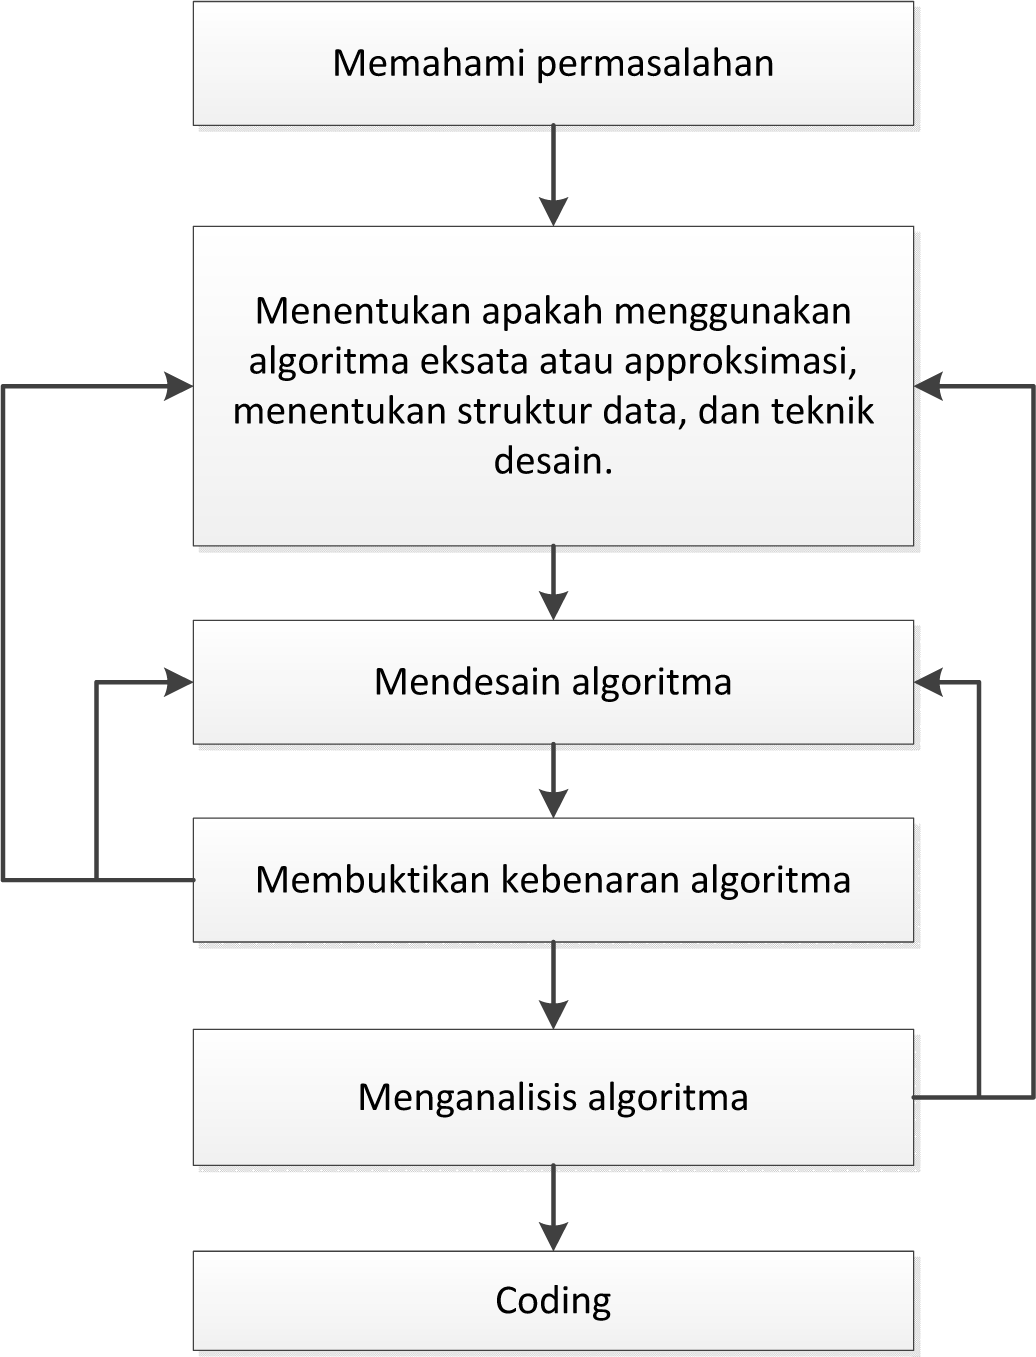
\includegraphics[scale=0.8]{fig/TahapanAnalisisDanDesain}
    \caption{Tahapan Analisis dan Desain Algoritma}
    \label{fig:TahapanAnalisisDanDesain}
\end{figure}

\subsection{Memahami permasalahan}
Memahami permasalahan merupakan langkah pertama dan merupakan langkah terpenting karena tanpa pemahaman yang baik langkah-langkah berikutnya tidak mungkin bisa terlaksana dengan baik. Pemahaman dilakukan dengan membaca deskripsi dari permasalahan secara baik. Apabila permasalahan tersebut merupakan permasalahan umum seperti misalnya masalah pengurutan, maka kita bisa menggunakan algoritma yang sudah ada untuk menyelesaikan. Jika tidak, maka kita harus mendesain dari awal algoritma tersebut.

Hal lain yang perlu diperhatikan baik-baik adalah masukan (\textit{input}) untuk permasalahan tersebut. Besarnya ukuran masukan menentukan algoritma yang akan kita gunakan. 

\subsection{Memilih antara penyelesaian permasalahan dengan pendekatan eksak (\textit{Exact}) atau approksimasi (\textit{Approximate})}
Yang dimaksud dengan pendekatan eksak adalah algoritma kita dijamin pasti bisa menemukan solusi dari permasalahan tersebut. Sedangkan pendekatan approksimasi, algoritma kita hanyalah memberikan hasil yang paling mendekati solusi sebenarnya. Kenapa perlu pendekatan approksimasi? Karena terkadang pendekatan eksak tidak bisa menemukan solusi dari permasalahan yang ada (bisa disebabkan karena ruang permasalahan sangat besar sekali sehingga memerlukan waktu yang sangat lama untuk menemukan solusinya).
 

\subsection{Menentukan struktur data}
Beberapa algoritma memerlukan struktur data tertentu seperti contohnya \textit{graph}. Struktur data yang tepat bisa memudahkan dan meningkatkan efisiensi waktu dan ruang dari implementasi sebuah algoritma tertentu. 

\subsection{Menentukan teknik desain algoritma}
Bagaimana jika permasalahan yang akan kita selesaikan tidak memiliki algoritma umum yang cocok untuk kita gunakan langsung? Maka kita harus mendesain algoritma tersebut dari awal. 

Untuk mendesain sebuah algoritma kita memerlukan teknik desain algoritma. Teknik desain algoritma merupakan sebuah pendekatan atau paradigma penyelesaian permasalahan yang bisa digunakan untuk berbagai jenis permasalahan yang ada. Salah satu contoh teknik desain algoritma adalah \textit{Divide and Conguer} dan \textit{Dynamic Programming}.

\subsection{Mendesain algoritma}
Jika kita sudah memahami permasalahan, menentukan struktur data dan teknik desain maka kita bisa melakukan desain algoritma. Desain algoritma bisa menggunakan bahasa perantara seperti \textit{pseudocode} atau \textit{flowchart}. Kita juga bisa langsung menggunakan bahasa pemrograman untuk mendesain algoritma. 

\subsection{Menentukan kebenaran dari algoritma}
Setelah sebuah algoritma selesai didesain, kita harus membuktikan kebenarannya atau dengan kata lain kita harus membuktikan bahwa algoritma kita memberikan solusi yang benar untuk semua masukan permasalahan dalam waktu yang terbatas. Ada beberapa cara untuk membuktikan kebenaran algoritma, salah satunya adalah menggunakan metode induksi matematika.

\subsection{Menganalisis algoritma}
Setelah mengetahui kebenaran dari sebuah algoritma maka langkah selanjutnya adalah mengetahui tingkat efisiensi ruang dan waktu dari algoritma tersebut. Efisiensi waktu menentukan seberapa cepat algoritma tersebut berjalan, sedangkan efisiensi ruang menentukan seberapa banyak memori yang diperlukan oleh algoritma tersebut. 

Untuk mengetahui seberapa effisien sebuah algoritma bisa dilakukan setelah menganalisis kompleksitas dari algoritma tersebut. Melakukan analisis algoritma berarti memprediksi berapa sumber daya (misalnya berapa lama waktu eksekusi atau berapa besar memori yang dibutuhkan) yang dibutuhkan oleh sebuah program ketika mengeksekusi algoritma tersebut. Pada umumnya, fokus analisis ditujukan pada waktu eksekusi dari algoritma tersebut walaupun tidak tertutup kemungkinan untuk menganalisi faktor lain.

\section{Pengenalan Kompleksitas Algoritma}
Hasil dari analisis biasanya berupa kompleksitas algoritma. Kita ambil contoh \textit{Insertion Sort}, dimana waktu yang diperlukan bagi \textit{Insertion Sort} untuk menyelesaikan proses pengurutannya tergantung pada jumlah masukan. Dengan kata lain, semakin besar jumlah masukan, semakin lama waktu yang diperlukan. Untuk dua masukan dengan jumlah yang sama, \textit{Insertion Sort} bisa memakan waktu yang berbeda tergantung dari seberapa terurutnya mereka. Dari sini, kita bisa mengambil kesimpulan bahwa, waktu yang diperlukan berkembang sesuai dengan ukuran dari masukan.

Besar masukan sebuah algoritma sangat tergantung terhadap permasalahan yang sedang dihadapi. Sebagai contohnya, jika berbicara mengenai permasalahan pengurutan maka besar masukan berupa berapa banyak bilangan dalam sebuah \textit{array} atau \textit{array size}. Untuk permasalahan lain seperti misalnya permasalahan pencarian rute terpendek dimana masukannya adalah berupa \textit{graph}, maka yang menjadi besar masukannya adalah jumlah \textit{vertice} dan \textit{edge} dari \textit{graph} tersebut. 

\section{Kompleksitas Algoritma}
Algoritma yang berbeda tentu saja memiliki langkah-langkah yang berbeda. Sehingga, ada algoritma yang lebih cepat dibandingkan algoritma yang lain. Dan ada pula algoritma yang lebih hemat dalam penggunaan memori. Algoritma yang baik adalah algoritma yang dapat menyelesaikan masalah  sekaligus efisien dalam pemakaian waktu dan ruang. Istilah yang digunakan untuk mengukur hal tersebut adalah \textbf{kompleksitas algoritma}. Maka, terdapat 2 jenis kompleksitas algoritma, yakni:

\begin{itemize}
    \item kompleksitas waktu ($T(n)$), dan
    \item kompleksitas ruang ($S(n)$).
\end{itemize}

Tentu diperlukan sebuah metode untuk mengukur seberapa cepat sebuah algoritma atau seberapa hemat pemakaian ruang memori dari algoritma tersebut. Menganalisis sebuah algoritma mencakup menganalisis kompleksitas algoritma. Meskipun terdapat 2 jenis kompleksitas, pada kuliah analisis dan desain algoritma ini yang lebih difokuskan adalah analisis kecepatan algoritma tersebut, atau kompleksitas waktunya ($T(n)$).

Cepat atau lambatnya sebuah algoritma tidak dihitung menggunakan satuan waktu yang umum digunakan dalam kehidupan, seperti detik, menit, ataupun jam. Alasannya karena kecepatan proses sebuah algoritma yang sudah diimplementasikan ke dalam program komputer bergantung pada banyak faktor, seperti prosessor, sistem operasi, \textit{compiler} yang digunakan, dan faktor lain. Menghitung kompleksitas waktu sebuah algoritma adalah \textbf{menghitung jumlah langkah yang ditempuh, serta perubahan jumlah langkah saat ukuran input berubah}. Jadi, tidak akan ada hubungannya dengan performa komputer atau kompiler yang digunakan sebagai media implementasi algoritma tersebut.

Pada banyak algoritma, jumlah langkah yang ditempuh sangat bergantung kepada ukuran dari masukan algoritma tersebut. Besar masukan sebuah algoritma sendiri sangat tergantung terhadap permasalahan yang sedang dihadapi. Sebagai contohnya, jika berbicara mengenai permasalahan pengurutan maka besar masukan berupa berapa banyak bilangan dalam sebuah \textit{array} (\textit{array size}). Untuk permasalahan lain seperti misalnya permasalahan pencarian rute terpendek dimana masukannya adalah berupa \textit{graph} (akan dijelaskan di mata kuliah struktur data), maka yang menjadi besar masukannya adalah jumlah \textit{vertice} dan \textit{edge} dari \textit{graph} tersebut. 


Banyaknya varian masukan serta cara perhitungan ukuran masukan yang berbeda-beda ini pada akhirnya menyebabkan perhitungan kompleksitas waktu algoritma memerlukan sebuah notasi khusus: \textbf{notasi asimtotik}.

\section{Notasi Asimtotik}

Sebagaimana dijelaskan pada sub-bagian di atas, untuk mengukur kompleksitas waktu algoritma tidak digunakan satuan waktu yang umum. Maka, dibutuhkan sebuah notasi khusus. Notasi matematis yang digunakan disebut \textbf{notasi asimtotik}. Notasi asimtotik digunakan untuk melihat seberapa efisien performa sebuah algoritma bila dibandingkan dengan algoritma yang lain. 

Terdapat beberapa jenis notasi asimtotik dalam bidang ilmu matematika yang digunakan dalam pengukuran kompleksitas algoritma. 3 contoh jenis notasi asimtotik adalah:

\begin{enumerate}
    \item O (Big-O)
    \item $\Omega$ (Big-Omega)
    \item $\Theta$ (Big-Theta)
\end{enumerate}

Dalam modul ini tidak akan dijelaskan secara terperinci bagaimana menggunakan masing-masing notasi. Namun, yang akan dijelaskan adalah bagaimana kompleksitas waktu sebuah algoritma dapat ditemukan dengan menggunakan notasi tersebut.

Notasi yang paling umum digunakan adalah O (Big-O). Alasannya adalah karena notasi tersebut digunakan untuk menggambarkan batas atas (\textit{upper limit}) dari sebuah fungsi ketika masukan untuk fungsi tersebut meningkat (\textit{increase}). Alhasil, Big-O sangat cocok untuk memperlihatkan \textit{worst case} dari sebuah algoritma. Apa yang dimaksud dengan worst case akan dijelaskan pada salah satu sub-bagian dari modul ini.

Contoh notasi Big-O: Algoritma Bubble Sort memiliki kompleksitas $T(n) = O(n^2)$. Artinya: algoritma Bubble Sort memiliki kompleksitas waktu $n^2$. 

\section{Mengukur Kompleksitas Algoritma Menggunakan Big-O}

Secara umum pengukuran kompleksitas algoritma dilakukan dengan melakukan perhitungan terhadap \textbf{pertumbuhan} jumlah langkah yang diperlukan untuk menyelesaikan sebuah algoritma. Biasanya langkah-langkah ini dihitung dengan cukup gamblang, yaitu dengan langsung menghitung berapa kali satu baris algoritma dijalankan.

Walaupun kedengarannya cukup mudah, perlu dicatat juga bahwa yang dijelaskan sebelumnya hanyalah cara menghitung kompleksitas algoritma non rekursif. Perhitungan kompleksitas algoritma non-rekursif tidak persis dengan algoritma rekursif. Untuk memulai pembahasan, kita akan membahas perhitungan kompleksitas pada algoritma non-rekursif terlebih dahulu. Kita baru akan membahas cara perhitungan kompleksitas algoritma rekursif pada bab berikutnya. Begitupun, dasar perhitungan kompleksitas adalah sama: menggunakan fungsi matematis dan aturan dasar penjumlahan.

Pada setiap modul, seraya berbagai teknik desain algoritma akan dibahas, juga akan diperlihatkan bagaimana menghitung kompleksitas algoritmanya. 

Secara umum, langkah-langkah untuk mengukur kompleksitas algoritma non-rekursif adalah sebagai berikut:

\begin{enumerate}
    \item Mengidentifikasi operasi dasar.
    \item Menentukan ukuran input.
    \item Memeriksa apakah pertumbuhan operasi dasar hanya bergantung pada ukuran input. Jika ya, maka tidak ada \textit{worst case} ataupun \textit{best case}. Namun jika terdapat faktor lain, maka perhitungan \textit{worst case} dibedakan dengan \textit{best case}.
    \item Menghitung derajat pertumbuhan langkah operasi dasar terhadap perubahan ukuran input dengan menggunakan fungsi matematika.
\end{enumerate}

Beberapa rumus matematika yang dapat digunakan untuk menunjang langkah keempat yaitu:

\begin{equation}\label{eq:common-1}
    \sum\limits_{i=l}^u 1 = 1 + 1 + 1 + 1 + \ldots = u - l + 1
\end{equation}

\begin{equation}\label{eq:common-2}
    \sum\limits_{i=1}^n 1 = n
\end{equation}

\begin{equation}\label{eq:common-3}
    \sum\limits_{i=1}^n i = 1 + 2 + \cdots + n = \frac{n(n + 1)}{2} \approx \frac{1}{2}n^2
\end{equation}

\begin{equation}\label{eq:common-4}
    \sum\limits_{i=1}^n i^2 = 1^2 + 2^2 + \cdots + n^2 = \frac{n(n + 1)(2n + 1)}{6} \approx \frac{1}{3}n^3
\end{equation}

\begin{equation}\label{eq:common-5}
    \sum\limits_{i=1}^n i^k = 1^k + 2^k + \cdots + n^k \approx \frac{1}{k + 1}n^{k+1}
\end{equation}

\begin{equation}\label{eq:common-6}
    \sum\limits_{i=0}^n a^i = 1 + a + \cdots + a^n = \frac{a^{n + 1} - 1}{a - 1}(a \neq 1)
\end{equation}

\begin{equation}\label{eq:common-7}
    \sum\limits_{i=0}^n 2^i = 2^{n + 1} - 1
\end{equation}

\begin{equation}\label{eq:common-8}
    \sum\limits_{i=1}^n i \times 2^i = 1 \times 2^1 + 2 \times 2^2 + \cdots + n \times 2^n \approx \frac{1}{3}n^3
\end{equation}

\begin{equation}\label{eq:common-9}
    \sum\limits_{i=l}^u ca_i = c \sum\limits_{i=l}^u a_i
\end{equation}

\begin{equation}\label{eq:common-10}
    \sum\limits_{i=l}^u (a_i \pm b_i) = \sum\limits_{i=l}{u} a_i \pm \sum\limits_{i=l}{u} b_i
\end{equation}

\begin{equation}\label{eq:common-11}
    \sum\limits_{i=m}^n 1 = n + 1 - m
\end{equation}

Biasanya kita akan mengubah deret langkah yang didapatkan melalui hasil perhitungan kompleksitas ke dalam bentuk yang lebih sederhana, dengan menggunakan fungsi-fungsi matematika di atas.

Untuk memperjelas, kita akan langsung mencoba melakukan perhitungan kompleksitas terhadap sebuah algoritma sederhana. Misalkan kita memiliki algoritma untuk menghitung nilai maksimum di dalam sebuah \textit{array} seperti berikut:

\lstinputlisting[language=Python, 
                 label={algo:maxelem},
                 caption=Maximum Element
                ]
                {code/1-max-element.py}

\FloatBarrier

Langkah-langkah yang dijalankan untuk menghitung kompleksitas yaitu:

\begin{enumerate}
    \item \textbf{Mengidentifikasi operasi dasar.} Operasi dasar adalah perbandingan antara \textbf{maximum} dan \textbf{arr[i]} pada baris ke 7, karena operasi ini merupakan operasi yang paling sering dilakukan yang merupakan logika dasar algoritma tersebut untuk memecahkan masalah.
    \item \textbf{Menentukan ukuran input.} Ukuran input adalah \textbf{arr\_len}, yang merupakan besar / panjang dari array atau list \textbf{arr}. \textbf{arr\_len} menjadi ukuran input karena berpengaruh terhadap banyaknya operasi dasar dilakukan.
    \item \textbf{Memeriksa apakah pertumbuhan operasi dasar hanya bergantung pada ukuran input.} Untuk algoritma pada listing~\ref{algo:maxelem}, \textbf{arr\_len} merupakan satu-satunya penentu banyaknya operasi dasar dilakukan, sehingga dalam perhitungan kompleksitas tidak diikutsertakan analisis \textit{worst case}, \textit{best case}, maupun \textit{average case}.
    \item \textbf{Menghitung derajat pertumbuhan langkah operasi dasar terhadap perubahan ukuran input dengan menggunakan fungsi matematika.} 
\end{enumerate}

Langkah keempat memerlukan perhitungan yang lebih mendetail. Derajat pertumbuhan yang dimaksud adalah seberapa besar pengaruh sebagian kode terhadap jumlah langkah keseluruhan dari sebuah algoritma. Pada algoritma dalam lsiting~\ref{algo:maxelem}, bagian yang mempengaruhi adalah bagian perulangan, tepatnya pada bagian yang diwarnai dalam listing~\ref{algo:maxelem-highlighted}.

\lstinputlisting[language=Python, 
                 caption=Perulangan pada Maximum Element, 
                 label={algo:maxelem-highlighted},
                 linebackgroundcolor={\ifnum\value{lstnumber}>5\ifnum\value{lstnumber}<11\color{codehighlight}\fi\fi}
                ]
                {code/1-max-element.py}

\FloatBarrier

Penjelasan: Perulangan merupakan deret, sehingga perulangan yang terpola dengan baik dapat digantikan ke dalam fungsi matematis berikut:

\begin{equation}\label{eq:maxelem-loop}
    T(n) = \sum\limits_{i=0}^{n-1} 1
\end{equation}

Isi dari sigma berisi 1 karena: \textbf{dalam setiap perulangan terdapat 1 kali operasi dasar yang dilakukan}. Selanjutnya, kita akan menggunakan rumus matematika~\ref{eq:common-1} pada fungsi~\ref{eq:maxelem-loop}:

\begin{equation}\label{eq:maxelem-loop-2}
T(n) = n - 1 + 1 = n
\end{equation}

Selanjutnya hasil akhir pada persamaan~\ref{eq:maxelem-loop-2} diubah ke dalam notasi asimtotik sesuai dengan aturan notasi seperti berikut:

$$
T(n) = O(n)
$$

Alhasil, algoritma di atas memiliki kompleksitas $O(n)$, atau sering disebut dengan kompleksitas linear.

\section{Kriteria Efisiensi umum}

Sebelum membahas lebih banyak contoh perhitungan kompleksitas lagi, kita akan terlebih dahulu melihat berbagai kriteria efisiensi algoritma yang ada. Terdapat beberapa kriteria efisiensi umum, yaitu:

\begin{enumerate}
    \item \textbf{$O (1)$: Kompleksitas Konstan.} Merupakan kriteria di mana ukuran input sama sekali tidak berpengaruh pada jumlah langkah sebuah algoritma. Kompleksitas ini merupakan jenis yang paling efisien / cepat.
        
    \begin{figure}
        \centering
        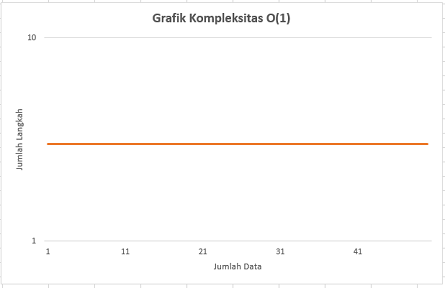
\includegraphics[width=\textwidth]{fig/ConstantGrowth}
        \caption{Grafik Pertumbuhan Konstan}
        \label{fig:ConstantGrowth}
    \end{figure}

    \FloatBarrier

    \item \textbf{$O (\log n)$: Kompleksitas Logaritmik.} Merupakan kompleksitas di mana perubahan / peningkatan besar dari ukuran input hanya memberikan sedikit sekali pengaruh terhadap pertumbuhan jumlah langkah. Algoritma yang memiliki kompleksitas logaritmik sering dijumpai pada algoritma yang dibuat dengan teknik divide \& conquer yang akan dibahas pada salah satu modul.

    \begin{figure}
        \centering
        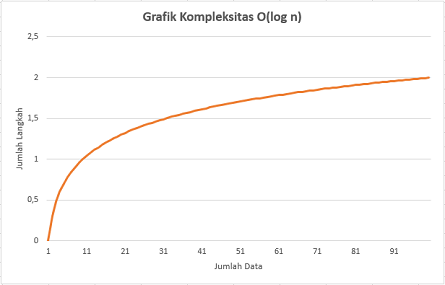
\includegraphics[width=\textwidth]{fig/LogarithmicGrowth}
        \caption{Grafik Pertumbuhan Logaritmik}
        \label{fig:LogarithmicGrowth}
    \end{figure}

    \FloatBarrier

    \item \textbf{$O (n)$: Linear.} Merupakan kompleksitas algoritma di mana pertumbuhan ukuran input sebanding dengan pertumbuhan jumlah langkah. Algoritma dengan kompleksitas linear dipandang sebagai algoritma yang cepat / efisien, meskipun itu juga bergantung pada permasalahan apa yang diselesaikan oleh sebuah algoritma.

    \begin{figure}
        \centering
        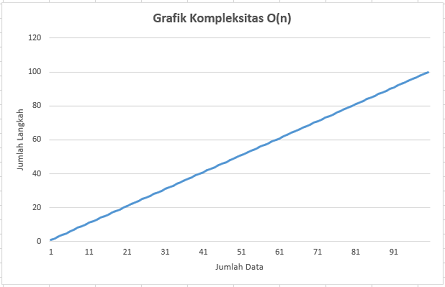
\includegraphics[width=\textwidth]{fig/LinearGrowth}
        \caption{Grafik Pertumbuhan Linear}
        \label{fig:LinearGrowth}
    \end{figure}

    \FloatBarrier

    \item \textbf{$O (n \log n)$.} Kompleksitas ini belum memiliki nama khusus. Jenis kompleksitas ini juga sering dijumpai pada algoritma yang berbasis teknik divide \& conquer. Hanya saja, pada kompleksitas jenis ini, perubahan jumlah langkah sedikit lebih besar daripada kompleksitas linear.

    \begin{figure}
        \centering
        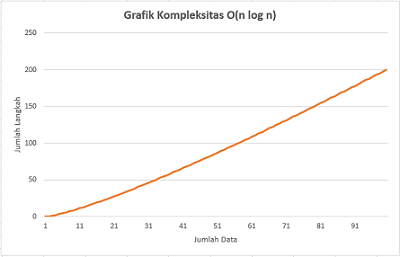
\includegraphics[width=\textwidth]{fig/NLogNGrowth}
        \caption{Grafik Pertumbuhan $n \log n$}
        \label{fig:NLogNGrowth}
    \end{figure}

    \FloatBarrier

    \item \textbf{$O (n^m)$: Kompleksitas Polinomial.} Merupakan jenis kompleksitas yang tinggi. $O (n^2)$ disebut dengan kompleksitas kuadratik. Merupakan jenis kompleksitas di mana sedikit perubahan pada ukuran input akan berpengaruh besar pada jumlah langkah.

    \begin{figure}
        \centering
        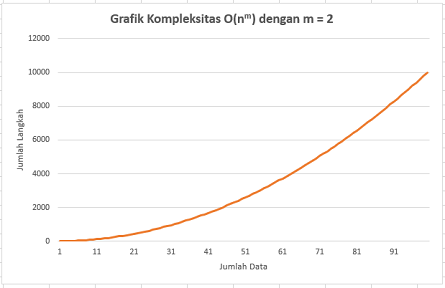
\includegraphics[width=\textwidth]{fig/ExponentialGrowth}
        \caption{Grafik Pertumbuhan Polinomial}
        \label{fig:ExponentialGrowth}
    \end{figure}

    \FloatBarrier

    \item \textbf{$O (n!)$: Kompleksitas faktorial.} Merupakan jenis kompleksitas yang sangat tinggi. Sedikit perubahan pada ukuran input akan berpengaruh sangat besar terhadap jumlah langkah. Kompleksitas ini sangat dihindari, namun untuk sebuah permasalahan komputasi yang sangat kompleks algoritma dengan kompleksitas yang tinggi juga sering digunakan.

    \begin{figure}
        \centering
        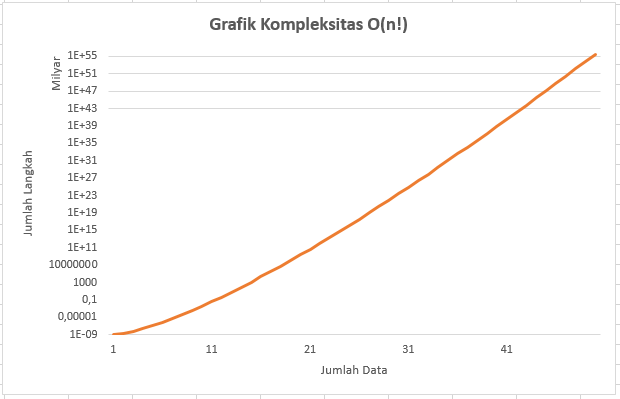
\includegraphics[width=\textwidth]{fig/FactorialGrowth}
        \caption{Grafik Pertumbuhan Faktorial}
        \label{fig:FactorialGrowth}
    \end{figure}

    \FloatBarrier
\end{enumerate}

Masing-masing kriteria efisiensi tersebut memiliki tingkat pertumbuhan yang berbeda-beda. Gambar~\ref{fig:allcomplexitycomparison} memperlihatkan perbandingan tingkat pertumbuhan dari masing-masing kriteria efisiensi. Perhatikan bagaimana $O(1)$ tak lagi terlihat di dalam gambar~\ref{fig:allcomplexitycomparison} karena nilainya yang sangat kecil (paling efisien).

\begin{figure}
    \centering
    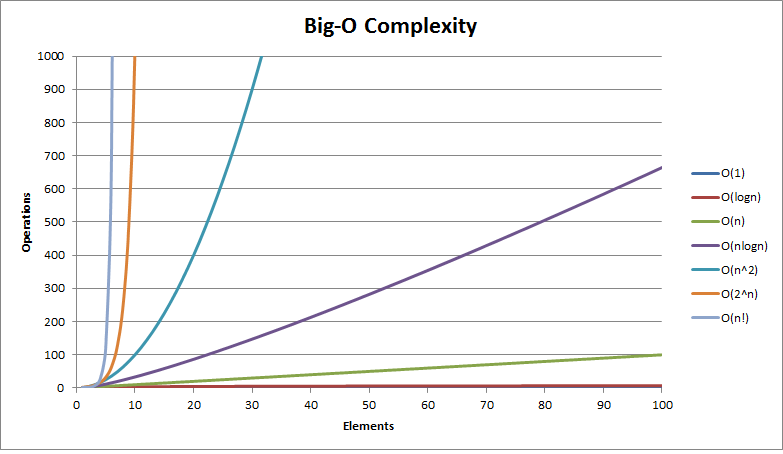
\includegraphics[width=\textwidth]{fig/AllComplexityComparison}
    \caption{Perbandingan Tingkat Pertumbuhan Seluruh Kriteria Efisiensi}
    \label{fig:allcomplexitycomparison}
\end{figure}

    \FloatBarrier

\section{Worst Case, Average Case, dan Best Case}

Dalam pengukuran kompleksitas algoritma, terdapat \textit{worst case}, \textit{average case}, dan \textit{best case}.

\begin{enumerate}
    \item Best case / kasus terbaik: merupakan kondisi di mana algoritma akan bekerja dengan kompleksitas paling rendah untuk ukuran input yang sama. Biasanya kasus \textit{best case} terjadi ketika algoritma menerima kondisi masukan yang optimal. Misalnya pada algoritma pengurutan, kondisi \textit{best case} dapat tercapai ketika kita memberikan masukan \textit{array} yang telah terurut. Hal ini memastikan algoritma akan berjalan dengan jumlah langkah minimal.
    \item Worst case / kasus terburuk: merupakan kebalikan dari kasus terbaik, di mana algoritma akan bekerja dengan kompleksitas tertinggi untuk ukuran input yang sama. Bertolak belakang dengan \textit{best case}, \textit{worst case} ditemukan ketika masukan sangat tidak optimal, sehingga algoritma harus berjalan dengan jumlah langkah maksimal.
    \item Average case / kasus rata-rata: merupakan kondisi yang paling sering terjadi untuk sebuah permasalahan.
\end{enumerate}

Pada prakteknya, pengukuran yang paling sering kita gunakan adalah pengukuran \textit{worst case} dan \textit{average case}. Begitupun, pengukuran \textit{best case} memiliki kegunaannya sendiri, misalkan pada kasus di mana kita mengetahui dengan persis seluruh masukan yang akan diterima.

\section{Contoh Kasus: Analisis Faktorial Iteratif}

Misalkan kita memiliki sebuah algoritma untuk menghitung faktorial dari sebuah bilangan sebagai berikut:

\lstinputlisting[language=Python, 
                 label={algo:faktorial},
                 caption=Algoritma Perhitungan Faktorial,
                 float
                ]
                {code/4-faktorial.py}

Kita dapat menghitung jumlah langkah yang harus dijalankan oleh algoritma~\ref{algo:faktorial} seperti berikut:

\begin{figure}%
    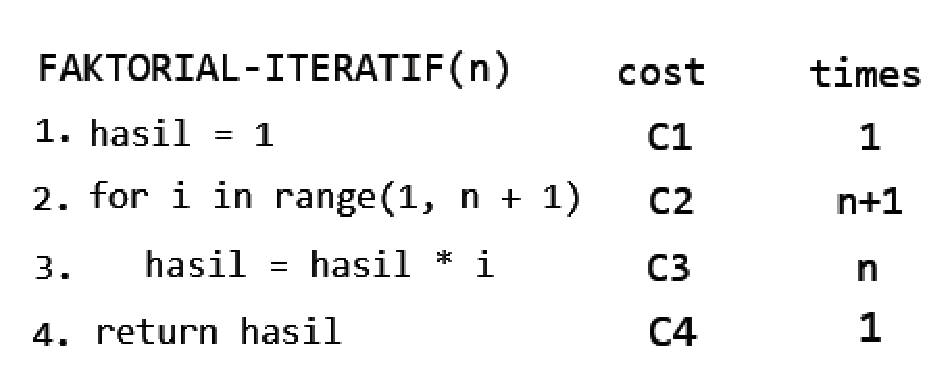
\includegraphics[scale=0.5]{fig/faktorialAnalysis}%
    \caption{Analisis Faktorial}%
    \label{fig:analisis-faktorial}%
\end{figure}

\FloatBarrier

Untuk mempermudah perhitungan, biasanya setiap langkah dianggap menghabiskan waktu yang konstan yaitu konstanta $c_i$ dimana $i$ menandakan baris keberapa dari \textit{pseudocode} algoritma tersebut. Nilai dari $c_i$ sendiri tidaklah penting, yang penting adalah berapa kali konstanta $c_i$ itu dieksekusi. Dari Gambar \ref{fig:analisis-faktorial}, setiap langkah (baris) memiliki biaya (\textit{cost}) eksekusi. 
Biaya eksekusi tersebut dilambangkan dengan besarnya konstanta $c_i$ yang dikalikan banyaknya konstanta tersebut dieksekusi yaitu $n$, dengan kata lain lamanya waktu yang dibutuhkan untuk mengeksekusi setiap langkah adalah $c_{i}\times{}n$ atau disingkat $c_{i}n$

Penjelasan lebih detil dari Gambar \ref{fig:analisis-faktorial} adalah sebagai berikut.

\begin{enumerate}
	\item Baris 1: Memiliki biaya sebesar $c_1$ dimana biaya tersebut akan diulang sebesar $1$ kali.  
	\item Baris 2: Memiliki biaya sebesar $c_2$ dimana biaya tersebut akan diulang sebesar $n+1$ kali. Pengulangan sebesar $n+1$ kali dikarenakan adanya sebuah looping ``\textbf{for i in range(1, n + 1)}''. Looping \textbf{for} akan dieksekusi oleh komputer sebanyak $n+1$ kali. Untuk mempermudah perhitungan maka kita misalkan $n$ bernilai 5, maka baris 2 akan diulang sebanyak 6 kali (1,2,3,4 dan 5 bernilai $True$ dan 1 kali terakhir bernilai $False$) atau $n$+1 kali.
	\item Baris 3: Memiliki biaya $c_{3}$. Ketiga baris tersebut masing-masing diulang sebanyak $n$ kali. Kenapa $n$ kali? Karena semua baris di dalam \textit{looping} \textbf{for} hanya diulang untuk setiap \textbf{for} yang bernilai $True$.
	\item Baris 4: Memiliki biaya 1 dan hanya berjalan 1 kali, yaitu ketika fungsi mengembalikan nilai ke pemanggilnya.
\end{enumerate}

Total waktu eksekusi dari Algoritma Faktorial Iteratif dilambangkan dengan $T(n)$ dimana:
\begin{equation}\label{eq:eksekusi-faktorial}
    \begin{aligned}
        T(n) &= c_{1} + c_{2}(n+1) + c_{3}n + c_{4}    \\ 
             &= c_{1} + c_{2}n + c_{2} + c_{3}n + c{4} \\
             &= (c_{2}+c_{3})n + (c_{1}+c_{2}+1)
    \end{aligned} 
\end{equation}

Persamaan \ref{eq:eksekusi-faktorial} bisa disederhanakan menjadi 

\begin{equation}\label{eq:faktorial-final}
    T(n) = an + b 
\end{equation}


Dari persamaan \ref{eq:faktorial-final} yaitu $an$ + $b$, terdapat dua konstan ($a$, dan $b$) yang besarnya tergantung pada $c_i$. Untuk membuat lebih sederhana, kita bisa membuat abstraksi yang lebih sederhana yaitu dengan hanya memperhatikan laju pertumbuhan fungsi (\textit{order of growth}). Untuk itu kita cukup hanya perlu memperhatikan order tertinggi dari fungsi yaitu $an$ karena order yang lebih rendah lajut pertumbuhannya tidak begitu signifikan untuk nilai $n$ yang besar.

Dengan perhitungan dan analisa di atas, dapat kita simpulkan bahwa algoritma faktorial di atas memiliki kompleksitas $O(n)$.

\section{Contoh Kasus: Analisis \textit{Bubble Sort}}

Sebagai contoh selanjutnya, kita akan melakukan analisa terhadap algoritma pengurutan nilai yang sangat sederhana dan naif: \textit{Bubble Sort}. Sebelum mulai melihat dan menganalisa algoritma, terlebih dahulu kita akan menentukan aturan dan batasan dari contoh kasus yang kita gunakan dalam modul ini.

Untuk mempermudah proses analisis, kita akan mengasumsikan bahwa algoritma yang diuji berjalan di sebuah komputer dengan prossesor tunggal dan \textit{random-access machine} (RAM). Model RAM yang kita adopsi adalah model yang menjalankan algoritma secara baris per baris instruksi tanpa ada proses parallel. 

Instruksi yang diperbolehkan untuk dijalankan pada umumnya adalah instruksi penjumlahan `+', pengurangan `-', perkalian `*', pembagian `/', modulus `\%', pembulatan atas `$\left\lceil\  \right\rceil$', dan pembulatan bawah `$\left\lfloor\ \right\rfloor$', penyimpanan/pengeluaran/duplikat data ke variabel (mis: $a = 5$ dan $a = b$), dan kontrol (IF, FOR, WHILE, RETURN dan sebagainya). Semua dari instruksi tersebut menggunakan waktu secara konstan (artinya memiliki nilai yang sama apapun kondisinya, kecuali disebutkan secara eksplisit).

Untuk setiap analisis, ada tiga jenis kasus yang mungkin terjadi, yaitu: kasus terbaik, kasus terburuk dan kasus rata-rata. Dalam pengurutan, kasus terbaik adalah ketika kita hendak mengurutkan rangkaian bilangan yang sudah terurut. Sedangkan kasus terburuk adalah ketika kita hendak mengurutkan rangkaian bilang yang terurut terbalik. Untuk kasus-kasus rangkaian bilang acak lainnya, kita gunakan kasus rata-rata.

Setelah aturan ditetapkan dengan benar, kita akan langsung mencoba melakukan analisa terhadap algoritma pertama, yaitu \textit{Bubble Sort}. Perhatikan implementasi algoritma \textit{Bubble Sort} berikut:

\lstinputlisting[language=Python, 
                 label={algo:bubble},
                 caption=Algoritma Bubble Sort,
                 float
                ]
                {code/2-bubble-sort.py}

Sebelum menganalisis Algoritma \ref{algo:bubble} ada dua hal penting yang harus dipahami terlebih dahulu: besar masukan (\textit{input size}) dan waktu eksekusi (\textit{running time}). 

\begin{figure}[htbp]%
	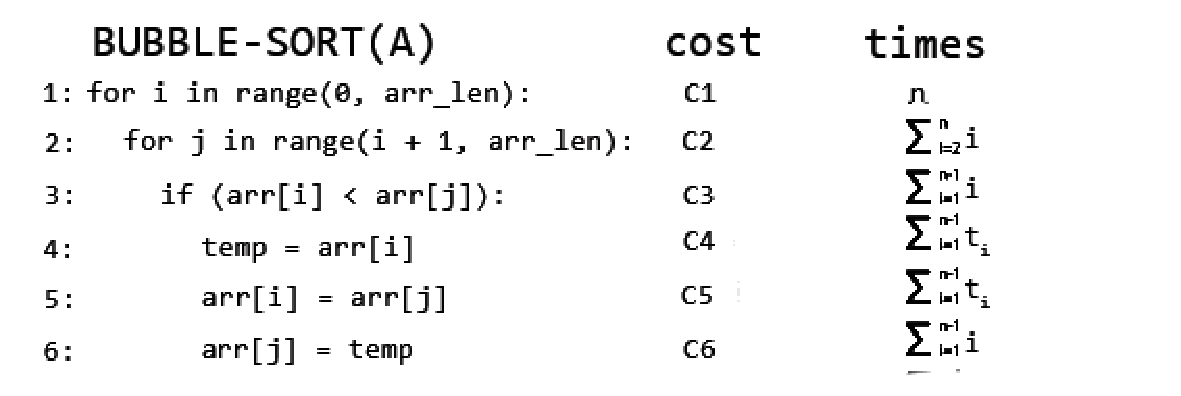
\includegraphics[scale=0.6]{fig/bubbleAnalysis.eps}%
	\caption{Analisis \textit{Bubble Sort}}%
	\label{fig:analisis-bubble-sort}%
\end{figure}

\FloatBarrier

Penjelasan lebih detil dari Gambar \ref{fig:analisis-bubble-sort} adalah sebagai berikut.

\begin{enumerate}
	\item Baris 1: Memiliki biaya sebesar $c_1$ dimana biaya tersebut akan diulang sebesar $n$ kali. Pengulangan sebesar $n$ kali dikarenakan looping \textbf{for} akan dieksekusi oleh komputer panjang arr\_len-1 + 1 kali.
	\item Baris 2: Baris ini diulang sebanyak $\sum\limits_{j=2}^n j$ kali. 
	\item Baris 3: Baris ini diulang sebanyak $\sum\limits_{j=1}^{n-1} j$ kali.
	\item Baris 4 - 6: Baris ini diulang sebanyak $\sum\limits_{j=1}^{n-1} t_{j}$ kali.
\end{enumerate} 

Total waktu eksekusi dari Algoritma \ref{algo:bubble} dilambangkan dengan $T(n)$ dimana:

\begin{equation}\label{eq:eksekusi-bubble-1}
    T(n) = c_{1}n + c_{2}\sum\limits_{j=2}^n j + c_{3}\sum\limits_{j=1}^{n-1} j + (c_{4}+c_{5}+c_{6})\sum\limits_{j=1}^{n-1} t_{j} 
\end{equation} 

Seandainya semua bilangan sudah terurut maka baris ke 4, 5 dan 6 dari Algoritma \ref{algo:bubble} tidak perlu dijalankan lagi karena perintah di baris ke 5 akan selalu menghasilkan $False$. Dengan kata lain nilai dari $t_{j}$ bernilai 0 karena tidak pernah dijalankan. Maka Persamaan \ref{eq:eksekusi-bubble-1} akan menjadi sebagai berikut.

\begin{equation}\label{eq:eksekusi-bubble-2}
    \begin{aligned}
        T(n) & = c_{1}n + c_{2}\sum\limits_{j=2}^n j + c_{3}\sum\limits_{j=1}^{n-1} j + (c_{4}+c_{5}+c_{6}) 0 \\
             & =  c_{1}n + c_{2}\sum\limits_{j=2}^n j + c_{3}\sum\limits_{j=1}^{n-1} j
    \end{aligned}
\end{equation}

Yang kemudian dengan menggunakan persamaan~\ref{eq:common-3} dapat kita sederhanakan menjadi:

\begin{equation}\label{eq:eksekusi-bubble-3}
    \begin{aligned}
        T(n) & =  c_{1}n + c_{2}\sum\limits_{j=2}^n j + c_{3}\sum\limits_{j=1}^{n-1} j \\
             & = c_{1}n + c_2 \frac{n(n+2)}{2} + c_3 \frac{n^2}{2} 
    \end{aligned}
\end{equation}

Persamaan \ref{eq:eksekusi-bubble-3} merupakan apa yang biasa disebut sebagai \textit{best case} atau kasus terbaik. Jika persamaan tersebut disederhanakan maka bisa ditulis sebagai $an^2+bn^2+c$. 

Untuk kasus terburuk (\textit{worst case}) akan terjadi jika \textit{array} angka yang akan diurut disusun secara terbalik semua (misalnya mengurut bilangan $\left\{5,4,3,2,1\right\}$ menjadi $\left\{1,2,3,4,5\right\}$). Untuk kasus tersebut, berarti kita harus mencocokkan setiap angka di \textit{inner loop}, atau dengan kata lain nilai dari $t_{j}$ adalah sama dengan nilai dari $j$. 

\begin{equation}\label{eq:eksekusi-bubble-4}
    T(n) = c_{1}n + c_2\frac{n(n+2)}{2} + (c_3+c_4+c_5+c_6)\frac{n^2}{2}
\end{equation}

Persamaan~\ref{eq:eksekusi-bubble-4} bisa disederhanakan menjadi $an^2+bn+c$ atau yang disebut juga dengan fungsi kuadratic akan $n$. 

Baik \textit{Best Case} dan \textit{Worst Case} sama-sama memiliki nilai $O(n^2)$.

\section{Contoh Kasus: Analisis \textit{Insertion Sort}}

Contoh ketiga masih menggunakan algoritma pengurutan, yaitu \textit{Insertion Sort}. Algoritma~\ref{algo:insertion} menunjukkan implementasi dari \textit{Insertion Sort}.

\lstinputlisting[language=Python, 
                 label={algo:insertion},
                 caption=Algoritma Insertion Sort
                ]
                {code/3-insertion-sort.py}

Waktu yang diperlukan bagi \textit{Insertion Sort} untuk menyelesaikan proses pengurutannya tergantung pada jumlah masukan. Dengan kata lain, semakin besar jumlah masukan, semakin lama waktu yang diperlukan. Untuk dua masukan dengan jumlah yang sama, \textit{Insertion Sort} bisa memakan waktu yang berbeda tergantung dari seberapa terurutnya mereka. Dari sini, kita bisa mengambil kesimpulan bahwa, waktu yang diperlukan berkembang sesuai dengan ukuran dari masukan.

Gambar~\ref{fig:analisis-insertion-sort} menunjukkan langkah-langkah analisis dari Algoritma \ref{algo:insertion}.

\begin{figure}[htbp]%
	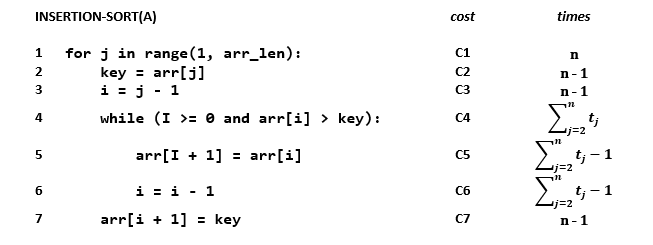
\includegraphics[scale=0.7]{fig/InsertionSortAnalysis.png}%
	\caption{Analisis \textit{Insertion Sort}}%
	\label{fig:analisis-insertion-sort}%
\end{figure}

\FloatBarrier

Penjelasan lebih detil dari Gambar \ref{fig:analisis-insertion-sort} adalah sebagai berikut.

\begin{enumerate}
	\item Baris 1: Memiliki biaya sebesar $c_1$ dimana biaya tersebut akan diulang sebesar $n$ kali. Pengulangan sebesar $n$ kali dikarenakan adanya sebuah looping ``for i in range(1, arr\_len)''. Looping \textbf{for} akan dieksekusi oleh komputer sebanyak arr\_len kali. Untuk mempermudah perhitungan maka kita lambangkan arr\_len sebagai $n$. Sebagai contohnya, jika arr\_len bernilai 5, maka baris 1 akan diulang sebanyak 6 kali (1,2,3,4 dan 5 bernilai $True$ dan 1 kali terakhir bernilai $False$) atau dengan kata lain $n$ bernilai 6.
	\item Baris 2 -- 3: Memiliki biaya masing-masing $c_{2}$ dan $c_{3}$. Kedua baris ini masing-masing diulang sebanyak $n-1$ kali. Kenapa $n-1$ kali? Karena semua baris di dalam \textit{looping} \textbf{for} hanya diulang untuk setiap \textbf{for} yang bernilai $True$.
	\item Baris 4: Baris ini diulang sebanyak $\sum\limits_{j=1}^n-1 t_{j}$ kali. Di baris ini ada dua buah \textit{looping}: \textit{outer loop} -- \textbf{for} dan \textit{inner loop} -- \textbf{while}. Untuk \textit{inner loop} dilambangkan dengan $t_{j}$. $t_{j}$ melambangkan jumlah \textit{looping inner loop}. Ketika \textit{inner loop} dan \textit{outer loop} digabungkan maka menjadi $\sum\limits_{j=1}^n-1 t_{j}$.  
\end{enumerate}                                       
                                     
Total waktu eksekusi dari Algoritma \ref{algo:insertion} dilambangkan dengan $T(n)$ dimana:

\begin{equation}\label{eq:eksekusi-insertion-1}
    T(n) = c_{1}n + c_{2}(n-1) + c_{4}(n-1) + c_{5}\sum\limits_{j=1}^n-1 t_{j} + c_{6}\sum\limits_{j=1}^n-1 (t_{j}-1) + c_{7}\sum\limits_{j=1}^n-1 (t_{j}-1) + c_{8}(n-1) 
\end{equation} 

Dari Persamaan \ref{eq:eksekusi-insertion-1}, kita bisa menghitung total waktu eksekusi ($T(n)$) yang bergantung kepada variabel $n$ atau banyaknya bilangan masukan. Semakin banyak bilangan masukan maka $T(n)$ akan semakin tinggi dan sebaliknya. Akan tetapi, $T(n)$ tidak hanya bergantung pada banyaknya bilangan masukan, tetapi bergantung juga kepada susunan bilangan tersebut. Bagaimana jika \textit{array} bilangan tersebut sudah terurut? Bukankah waktu yang dibutuhkan akan lebih sedikit dibandingkan jika semua bilangan tersebut terbalik urutannya?

Seandainya semua bilangan sudah terurut maka baris ke 5 dan baris ke 6 dari Algoritma \ref{algo:insertion} tidak perlu dijalankan lagi karena perintah di baris ke 4 akan selalu menghasilkan $False$. Dengan kata lain nilai dari $t_{j}$ akan selalu konstan yaitu 1. Maka Persamaan \ref{eq:eksekusi-insertion-1} akan menjadi sebagai berikut:

\begin{equation}\label{eq:insertion-sort-optimal}
    \begin{aligned}
        T(n) & = c_{1}n + c_2(n-1)+c_4(n-1)+c_5(n-1)+c_8(n-1) \\
             & = (c_1+c_2+c_4+c_5+c_8)n-(c_2+c_4+c_5+c_8)
    \end{aligned}
\end{equation}

Persamaan \ref{eq:insertion-sort-optimal} merupakan apa yang biasa disebut sebagai \textit{best case} atau kasus terbaik. Jika persamaan tersebut disederhanakan maka bisa ditulis sebagai $an+b$ atau yang biasa disebut sebagai fungsi linear akan $n$. 

Untuk kasus terburuk (\textit{worst case}) akan terjadi jika \textit{array} angka yang akan diurut disusun secara terbalik semua (misalnya mengurut bilangan $\left\{5,4,3,2,1\right\}$ menjadi $\left\{1,2,3,4,5\right\}$). Untuk kasus tersebut, berarti kita harus mencocokkan setiap angka di \textit{inner loop}, atau dengan kata lain nilai dari $t_{j}$ adalah sama dengan nilai dari $j$ yang berasal dari \textit{outer loop}. 

\begin{equation}\label{eq:eksekusi-insertion-sort-2}
    \begin{aligned}
        T(n) & = c_1n + c_2(n-1) + c_4(n-1) + c_5(\frac{n(n+1)}{2}-1) + c_6(\frac{n(n-1)}{2}) \\ 
             &   + c_7(\frac{n(n-1)}{2})+c_8(n-1) \\
             & = (\frac{c_5}{2}+\frac{c_6}{2}+\frac{c_7}{2})n^2+(c_1+c_2+c_4+\frac{c_5}{2}-\frac{c_6}{2}-\frac{c_7}{2}+c_8)n \\
             &   -(c_2+c_4+c_5+c8)
    \end{aligned}
\end{equation}

Persamaan \ref{eq:eksekusi-insertion-sort-2} bisa disederhanakan menjadi $an^2+bn+c$ atau yang disebut juga dengan fungsi kuadratic akan $n$. 

Dari persamaan \ref{eq:eksekusi-insertion-sort-2} yaitu $an^2+bn+c$, terdapat tiga konstan ($a$, $b$, dan $c$) yang besarnya tergantung pada $c_i$. Untuk membuat lebih sederhana, kita bisa membuat abstraksi yang lebih sederhana yaitu dengan hanya memperhatikan laju pertumbuhan fungsi (\textit{order of growth}). Untuk itu kita cukup hanya perlu memperhatikan order tertinggi dari fungsi yaitu $an^2$ karena order yang lebih rendah lajut pertumbuhannya tidak begitu signifikan untuk nilai $n$ yang besar. Untuk itu kita tulis bahwa \textit{insertion sort} memiliki \textit{worst case} $O(n^2)$.


%\chapter{Teknik \textit{Greedy}}

Algoritma greedy merupakan Algoritma greedy merupakan metode yang paling populer untuk memecahkan persoalan optimasi. Optimisasi adalah suatu proses untuk mencapai hasil yang optimal (nilai optimal/efektif yang dapat dicapai). Sedangkan yang dimaksud dengan nilai optimal adalah nilai yang didapat melalui suatu  proses dan dianggap menjadi solusi jawaban yang paling baik dari semua solusi yang ada. Pada kebanyakan kasus, algoritma greedy tidak akan menghasilkan solusi paling optimal, tetapi algoritma greedy biasanya memberikan solusi yang mendekati nilai optimum dalam waktu yang cukup cepat. 

Persoalan optimasi (optimization problem) adalah persoalan yang menuntut pencarian solusi optimum. Persoalan optimasi dibagi menjadi dua macam, yaitu maksimasi (maximization) dan minimasi (minimization). Solusi optimum merupakan solusi yang bernilai minimum atau maksimum dari sekumpulan alternatif solusi yang mungkin yang diperoleh. 

Contoh dari permasalahan optimasi dapat berupa penukaran uang. Misalkan untuk menukarkan uang senilai 32 sen dengan sekumpulan uang koin. Berapa jumlah minimum koin yang diperlukan tersebut jika koin-koin yang tersedia bernilai 11, 7, 3, dan 2. 

Algoritma greedy sendiri adalah algoritma yang memecahkan masalah langkah per langkah, pada setiap langkah mengambil pilihan yang terbaik yang dapat diperoleh pada saat itu tanpa memperhatikan konsekuensi ke depan ( \textquotedblleft take what you can get now!\textquotedblright ) dan	berharap bahwa dengan memilih optimum lokal pada setiap langkah akan berakhir dengan optimum global.

Strategi greedy yang digunakan untuk menyelesaikan masalah penukaran uang senilai 32 sen dengan sekumpulan koin bernilai 11, 7, 3, dan 2 adalah :

\begin{enumerate}
\item Pada setiap langkah, pilihlah koin dengan nilai yang paling besar dari himpunan koin yang tersisa dengan syarat tidak melebihi nilai uang yang ditukarkan.
\item	Agar pemilihan koin optimal, maka perlu mengurutkan himpunan koin dalam urutan yang menurun. 
\item	Jika himpunan koin sudah terurut menurun, maka kompleksitas algoritma greedy adalah O(n). Jika waktu pengurutan diperhitungkan, maka kompleksitas algoritma greedy ditentukan dari kompleksitas algoritma pengurutan himpunan koin. 

\end{enumerate}

Langkah 1: pilih 1 buah koin 11  (Total = 11)

Langkah 2: pilih 1 buah koin 11   (Total = 11 + 11 = 22)
	
Langkah 3: pilih 1 buah koin 7  (Total = 22 + 7= 29)  

Langkah 4: pilih 1 buah koin 3  (Total = 29 + 3 = 32)  

Solusi: Jumlah koin minimum = 4 (solusi optimal!)

Pada setiap langkah di atas akan diperoleh optimum lokal, dan pada akhir algoritma akan diperoleh optimum global (yang pada contoh ini merupakan solusi optimum).

Algoritma \textit{Greedy} dalam bahasa Python diterapkan dalam menyelesaikan penukaran uang seperti berikut ini:

\lstset{language=Python}
\label{lst:CoinchangeProblem}
\begin{lstlisting}[frame=single]
def tukar(jumlah):
 koin = [11,7,3,2]
 hasil = 0 
 i = 0
 while (jumlah != 0) and (i < len(koin)):
  if(jumlah - koin[i] < 0):
   i=i+1
  else
   jumlah = jumlah - koin[i]
   hasil = hasil + 1
			
 if(jumlah > 0) :  
  print "koin tidak bisa ditukar"
 else :
  print  "Hasil : ", hasil + " koin didapatkan"
	
\end{lstlisting}

Algoritma greedy untuk masalah penukaran uang ini  tidak selalu memberikan hasil yang optimal, bergantung pada koin mata uang yang digunakan. 
\begin{flushleft}
Contoh :\break
\break
(a)Koin: 5, 4, 3, dan 1 dengan jumlah uang yang ditukar = 7.
\break
Solusi dengan algoritma greedy: 7 = 5 + 1 + 1		=	( 3 koin)  tidak optimal
\break
Solusi yang optimal: 7 = 4 + 3	( 2 koin)
\break
\break
(b)  Koin: 10, 7, 2 dengan jumlah uang yang ditukar: 16
\break
Solusi dengan algoritma greedy: 16 = 10 + 2 + 2 + 2 (4 koin)
\break
Solusi yang optimal: 16 = 7 + 7 + 2	(hanya 3 koin)
\break
\break
(c) Koin: 15, 10, dan 1 dengan jumlah uang yang ditukar: 21
\break
Solusi dengan algoritma greedy: 21 = 15 + 1 + 1 + 1 + 1 + 1	+ 1(7 koin)
\break
Solusi opgtimal: 21 = 10 + 10	+ 1	(3 koin)
\break
\end{flushleft}
%•	Untuk sistem mata uang dollar AS, euro Eropa, dan crown Swedia, algoritma greedy selalu memberikan solusi optimum. Misalnya untuk menukarkan $6,39 dengan uang kertas (bill) dan koin sen (cent), kita dapat memilih:
%•	Satu buah uang kertas senilai $5	
%•	Satu buah uang kertas senilai $1 ($5 + $1 = $6))
%•	Satu koin  25 sen	($5 + $1 + 25c = $6,25)
%•	Satu koin 10 sen	($5 + $1 + 25c + 10c = $6,35)
%•	Empat koin 1 sen	($5 + $1 + 25c + 10c + 1c + 1c + 1c + 1c = $6,39)
	%
%Bagaimana dengan mata uang rupiah Indonesia? 

Ada kalanya optimum global dari greedy algoritma merupakan solusi sub-optimum dari sebuah masalah. Alasan:
\begin{enumerate}
\item algoritma greedy tidak beroperasi secara menyeluruh terhadap semua alternatif solusi yang ada.  
\item	pemilihan fungsi SELEKSI: beberapa fungsi SELEKSI yang berbeda dapat menghasilkan solusi yang berbeda 
\end{enumerate}

Karena itu, pada sebagian masalah algoritma greedy, tidak selalu dapat memberikan solusi yang  optimum. Akan tetapi, jika nilai optimum tidak diperlukan, maka algoritma greedy sangat berguna untuk menghasilkan solusi yang menghampiri (approximation) optimum, daripada menggunakan algoritma yang lebih rumit untuk menghasilkan solusi yang eksak. 

\section{\textit{Pohon Huffman (Huffman Tree)}}

\textit{Kode Huffman} adalah kumpulan string biner yang digunakan untuk mengkodekan setiap karakter. Kode Huffman pada dasarnya merupakan kode prefiks (prefiks code), yaitu berisi sekumpulan kode biner yang dalam hal ini tidak ada kode biner yang menjadi awal bagi kode biner yang lain.

Kode prefiks dapat direpresentasikan dengan pohon biner yang diberi nilai 0 (cabang kiri) dan 1 (cabang kanan). Rangkaian bit yang terbentuk pada setiap lintasan dari akar sampai tree merupakan kode prefiks untuk karakter setiap karakter.

Penggunaan algoritma greedy pada algoritma Huffman ada pada saat pemilihan dua pohon dengan frekuensi terkecil dalam membuat pohon Huffman. Algoritma greedy digunakan untuk meminimumkan total cost yang dibutuhkan dalam pembuatan pohon Huffman. Cost yang digunakan untuk menggabungkan dua buah pohon pada akar setara dengan jumlah frekuensi dua buah pohon yang digabungkan, oleh karena itu total cost pembentukan pohon Huffman adalah jumlah total seluruh penggabungan. Penggabungan dua buah pohon dilakukan setiap langkah dan algoritma Huffman selalu memilih dua buah pohon yang mempunyai frekuensi terkecil untuk meminimumkan total cost. Oleh karena itu algoritma Huffman adalah salah satu contoh algoritma yang menggunaan dari algoritma Greedy.

Langkah-langkah pembentukan pohon Huffman adalah sebagai berikut:
\begin{enumerate}
\item Hitung frekuensi kemunculan karakter didalam data. Setiap karakter dinyatakan sebagai pohon bersimpul tunggal. Setiap simpul di-assign dengan frekuensi kemunculan karakter.
\item Terapkan algorithma Greedy yaitu dengan menggabungkan dua buah pohon yang mempunyai frekuensi terkecil pada sebuah akar. Setelah digabungkan akar tersebut akan mempunyai frekuensi yang merupakan jumlah dari frekuensi dua buah pohon-pohon penyusunnya.
\item Ulangi langkah 2 sampai hanya tersisa satu buah pohon Huffman. Agar pemilihan dua pohon yang akan digabungkan berlangsung cepat, maka semua harus terurut naik berdasarkan frekuensinya.
\end{enumerate}
Sebagai contoh kode Huffman diterapkan pada bahasa prancis "j'aime aller sur le bord de l'eau les jeudis ou les jours impairs" akan didapatkan frikuensi kemunculan seperti Tabel 1.1.

\begin{table}[h]
\begin{center}
\begin{tabular}{|c|c|c|c|c|c|c|c|c|c|c|c|c|c|c|}
\hline
b&p&'&m&j&o&d&a&i&r&u&l&s&e&space\\
\hline
1&1&2&2&3&3&3&4&4&5&5&6&6&8&12\\
\hline
\end{tabular}
\caption{Frekuensi Kemunculan}
\end{center}
\end{table}

Akan dihasilkan pohon Huffman sebagai berikut:

\begin{figure}[htbp]
\begin{center}
	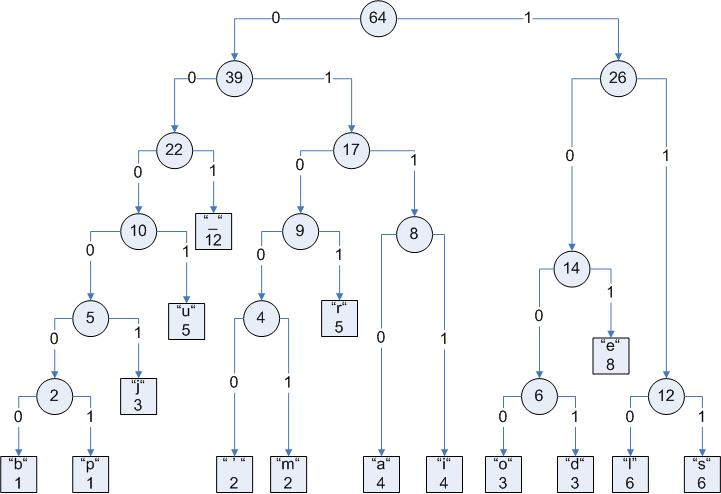
\includegraphics[scale=0.6]{fig/sunario-3/Huffman.jpg}%
	\caption{Hasil pohon }%
	\label{fig:Huffman Tree}%
\end{center}
\end{figure}

Pohon Huffman berfungsi pada proses Encoding dan Decoding data dengan syarat bahwa encoder dan decoder sudah sepakat untuk menggunakan Huffman tree tertentu sebelum terjadi pengiriman data. Encoder membangun Huffman tree yang baru setiap data baru akan dikirimkan, dan mengirimkan tabel konversi bersama-sama dengan data.

Untuk Algoritma Huffman mempunyai kompleksitas $O(n log n)$ untuk himpunan dengan n karakter.	

\section{\textit{Knapsack Problem}}

\textit{Knapsack Problem} merupakan suatu permasalahan bagaimana memilih objek dari sekian banyak dan  berapa besar objek tersebut akan disimpan sehingga diperoleh suatu penyimpanan yang optimal dengan memperhatikan objek yang terdiri dari n objek (1,2,3,...) dimana setiap objek memiliki  bobot (Wi) dan profit (Pi) dengan memperhatikan juga kapasitas dari media penyimpanan sebesar M dan nilai probabilitas dari setiap objek (Xi). Contoh permasalahan ini dalam dunia nyata adalah pedagang keliling dengan menggunakan gerobak ataupun alat pengangkut lainnya yang hanya memiliki kapasitas angkut maksimum sebesar w kg barang yang akan dijual.Barang yang dijual berjumlah satu untuk tiap jenisnya dan tiap jenis barang memiliki berat w1,w2,w3,w4, ..wn dengan keuntungan yang diperoleh untuk tiap jenisnya adalah p1,p2,p3,p4, .pn. Tetapi tidak semua jenis barang yang akan dijual oleh pedagang keliling tersebut dapat dimasukan kedalam alat pengangkut. Maka akan dipilih jenis-jenis barang yang akan dijual untuk setiap harinya oleh pedagang keliling tersebut agar diperoleh keuntungan yang maksimal dari penjualan barang-barang  tersebut. 

\subsection{Knapsack $0/1$}
knapsack 0/1, merupakan suatu masalah untuk memilih objek diambil, dengan ketentuan objek yang diambil harus seluruh diambil atau tidak sama sekali. Setiap   objek  tersebut mempunyai   nilai   keuntungan   atau   yang   disebut   dengan   profit.	Tujuan dari profit tersebut adalah untuk mendapatkan profit   yang   maksimal. Untuk   mendapatkan profit maksimal, tidak dapat ditentukan dari  banyak   objek   yang   masuk. Bisa saja hal yang sebaliknya yang terjadi. 

\begin{table}[h]
\begin{center}
\begin{tabular}{|c|c|c|c|}
\hline
W1 & 3  & p1 & 12 \\
W2 & 6  & p2 & 18\\
W3 & 5  & p3 & 10\\
W4 & 10  & p4 & 50\\
\hline
\multicolumn{4}{ |c| }{W maksimal = 16}\\
\hline
\end{tabular}
\caption{Data Masukkan}
\end{center}
\end{table}

Pada algoritma Greedy ada beberapa strategi yang digunakan untuk memilih objek yang akan dimasukkan kedalam knapsack seperti table 1.1 diatas, yaitu:
\begin{enumerate}
\item Greedy by profit \newline
Pada setiap langkah, knapsack diisi dengan objek yang mempunyai keuntungan terbesar. Strategi ini mencoba memaksimumkan keuntungan dengan memilih objek yang paling menguntungkan terlebih dahulu.

Pertama kali dilakukan adalah menurutkan secara menurun obyek-obyek berdasarkan profitnya .  Kemudian obyek-obyek yang dapat ditampung oleh knapsack diambil satu persatu sampai knapsack penuh atau (sudah tidak ada obyek lagi yang bisa dimasukan).
\begin{table}[h]
\begin{center}
\begin{tabular}{|c|c|c|c|c|}
\hline
\multicolumn{5}{ |c| }{Objek}\\
\hline
i & wi  & pi & pi/wi & status \\
\hline
4 & 10  & 50 & 5 & 1 \\
2 & 6  & 18 & 3 & 1 \\
3 & 5  & 10 & 2 & 0 \\
1 & 3  & 12 & 4 & 0 \\
\hline
\end{tabular}
\caption{Greedy by profit}
\end{center}
\end{table}
\item Greedy by weight.\newline
Pada setiap langkah, knapsack diisi dengan objek yang mempunyai berat paling ringan. Strategi ini mencoba memaksimumkan keuntungan dengan memasukkan sebanyak mungkin objek ke dalam knapsack.

Pertama kali yang dilakukan adalah mengurutkan secara menaik objek-objek berdasarkan weight-nya. Kemudian obyek-obyek yang dapat ditampung oleh knapsack diambil satu persatu sampai knapsack penuh atau (sudah tidak ada obyek lagi yang bisa dimasukan).
\begin{table}[h]
\begin{center}
\begin{tabular}{|c|c|c|c|c|}
\hline
\multicolumn{5}{ |c| }{Objek}\\
\hline
i & wi  & pi & pi/wi & status \\
\hline
1 & 3  & 12 & 4 & 1 \\
3 & 5  & 10 & 2 & 1 \\
2 & 6  & 18 & 3 & 1 \\
4 & 10  & 50 & 5 & 0 \\
\hline
\end{tabular}
\caption{Greedy by weight}
\end{center}
\end{table}
\item   Greedy by density. \newline
Pada setiap langkah, knapsack diisi dengan objek yang mempunyai densitas,  $pi / wi$ terbesar. Strategi ini mencoba memaksimumkan keuntungan dengan memilih objek yang mempunyai keuntungan per unit berat terbesar.

Pertama kali yang dilakukan adalah mencari nilai profit per unit/ density dari tiap-tiap objek. Kemudian obyek-obyek diurutkan berdasarkan densitasnya.
Kemudian obyek-obyek yang dapat ditampung oleh knapsack diambil satu persatu sampai knapsack penuh atau (sudah tidak ada obyek lagi yang bisa dimasukan).

\begin{table}[h]
\begin{center}
\begin{tabular}{|c|c|c|c|c|}
\hline
\multicolumn{5}{ |c| }{Objek}\\
\hline
i & wi  & pi & pi/wi & status \\
\hline
4 & 10  & 50 & 5 & 1 \\
1 & 3  & 12 & 4 & 1 \\
2 & 6  & 18 & 3 & 0 \\
3 & 5  & 10 & 2 & 0 \\
\hline
\end{tabular}
\caption{Greedy by weight}
\end{center}
\end{table}
\end{enumerate}

Perbandingan hasil optimal Penggunaan 3 strategi diatas Hal dapat dilihat pada tabel 1.5 berikut ini:

\begin{table}[h]
\begin{center}
\begin{tabular}{|c|c|c|c|c|c|c|c|}
\hline
\multicolumn{4}{ |c| }{Objek} & \multicolumn{3}{|c|}{Greddy by}  & \multirow{2}{*}{Solusi Optimal} \\
\hline 
i & wi  & pi & pi/wi & profit & weight & density \\
\hline
1 & 3  & 12 & 4 & 0 & 1 & 1 & 0\\
2 & 6  & 18 & 3 & 1 & 1 & 0 & 1\\
3 & 5  & 10 & 2 & 0 & 1 & 0 & 0\\
4 & 10  & 50 & 5 &1 & 0 & 1 & 1\\
\hline
\multicolumn{4}{ |r| }{Total Bobot} &16 & 14 & 13 & 16\\
\hline
\multicolumn{4}{ |r| }{Total Keuntungan} &68 & 40 & 62 & 68\\
\hline
\end{tabular}
\caption{}
\end{center}
\end{table}

Algoritma \textit{knapsack 0/1} dalam bahasa phyton dapat dituliskan sebagai berikut :

\lstset{language=Python}
\label{lst:Knapsack 0/1}
\begin{lstlisting}[frame=single]
def knapsack(v,w,n,W):
 V = [[for x in range(W+1)] for x in range(len(v)+1)]
 for j in range(W+1):
  V[0][j] = 0
	
 for i in range(1,n+1):
  for wx in range(W+1):
   if w[i-1] <= wx:
    V[i][wx] = max(V[i-1][wx], v[i-1]+V[i-1][wx-w[i-1]])
   else:
    V[i][wx] = V[i-1][wx]
		
 return V[n][W] 
\end{lstlisting}

Kompleksitas waktu algoritma di atas (dengan mangabaikan waktu pengurutan objek) adalah O(nW). 

\subsection{Fractional Knapsack}

Berbeda dengan knapsack 0/1, Fractional Knapsack merupakan suatu masalah untuk memilih objek diambil, dengan ketentuan objek hanya dapat diambil sebagian. Algoritma Greedy dalam hal ini memperoleh solusi dari masalah dengan membuat urutan pilihan. Ide dasarnya adalah untuk menghitung  rasio untuk setiap objek berdasarkan   bobot (Wi)  / profit (Pi) (Wi/Pi), dan diurutkan sesuai dengan rasionya. Kemudian objek dengan rasio tertinggi ditambahkan sampai objek tidak dapat diambil lagi. 

Sebagai contoh:\newline

\begin{table}[h]
\begin{center}
\begin{tabular}{|c|c|c|c|}
\hline
w1 & 18&    p1 & 25 \\
w2 & 15&    p2 & 24 \\
w3 & 10&    p3 & 15 \\
\hline
\multicolumn{4}{ |c| }{W maksimal = 20}\\
\hline
\end{tabular}
\caption{Data Masukkan}
\end{center}
\end{table}

Solusi dengan algoritma greedy dalam penyelesaian persoalan knapsack yang memakai strategi pemilihan objek berdasarkan pi /wi terbesar memberikan keuntungan yang maksimum (optimum). Agar proses pemilihan objek berikutnya optimal, maka kita perlu mengurutkan objek terlebih dahulu berdasarkan pi /wi dalam urutan yang menurun,  sehingga objek berikutnya yang dipilih adalah objek sesuai dalam urutan

\begin{table}[h]
\begin{center}
\begin{tabular}{|c|c|c|c|c|c|c|}
\hline
\multicolumn{4}{ |c| }{Objek} & \multicolumn{3}{|c|}{Greddy by}  \\
\hline 
i & wi  & pi & pi/wi & profit & weight & density \\
\hline
2 & 15 & 24 & 1,6 & $2/15$ & $2/3$ & 1\\
3 & 10 & 15 & 1,5 & 0 & 1 & $1/2$ \\
1 & 18 & 25 & 1,4 & 1 & 0 & 0 \\

\hline
\multicolumn{4}{ |r| }{Total Bobot} &20 & 20 & 20 \\
\hline
\multicolumn{4}{ |r| }{Total Keuntungan} &28,2 & 31,0 & 31,5 \\
\hline
\end{tabular}
\caption{Tabel Hasil Fractional Knapsack}
\end{center}
\end{table}

Solusi optmal persoalan knapsack di atas adalah X = (0, 1, 1/2) yang dimana dapat memberikan keuntungan maksimum 31,5.

Algoritma \textit{Fractional Knapsack} dalam bahasa phyton dapat dituliskan sebagai berikut :

\lstset{language=Python}
\label{lst:Fractional Knapsack}
\begin{lstlisting}[frame=single]
def knapsack(v,w,W):
 x=[]
 weight = 0
 i=0;
 while(weight<W):
  if(weight+w[i]<=w):
	 x[i]=1;
	 weight = weight +w[i]
	else:
	 x[i] = (w-weight)/w[i]
	 weight = W
 i+=1;
return x 
\end{lstlisting}

Kompleksitas waktu algoritma di atas (dengan mangabaikan waktu pengurutan objek) adalah O(n). 

\section{\textit{Algoritma Dijkstra}}
Salah satu permasalahan yang berkaitan dengan optimisasi adalah menentukan lintasan terpendek dari suatu tempat ke tempat yang lain.Permasalahan ini dapat diselesaikan dengan sebuah metode yang menggunakan perhitungan matematika eksak yaitu Algoritma Dijkstra.

Algoritma Dijkstra adalah algoritma dijkstra beroperasi secara menyeluruh terhadap semua alternatif fungsi yang ada sehingga rute terpendek yang didapat hanya dari titik awal sampai titik tujuan. Algoritma ini menggunakan prinsip greedy. Prinsip greedy pada algoritma dijkstra menyatakan bahwa pada setiap langkah,  pilih sisi yang berbobot minimum dan memasukannya dalam himpunan solusi. Cara kerja dari algoritma dijkstra adalah sebagai berikut:
\begin{enumerate}
\item Pada awalnya pilih sisi dengan bobot terendah dari node yang belum terpilih, diinisialisasi dengan 0 dan yang sudah terpilih diinisialisasi dengan 1.
\item Bentuk tabel yang terdiri dari titik ,status, bobot dan predecessor. Lengkapi kolom bobot yang diperoleh dari jarak titik sumber ke semua titik yang terhubung langsung dengan titik sumber tersebut
\item Jika titik sumber telah ditemukan maka tetapkanlah titik tersebut sebagai titik pilihan.
\item Tetapkan titik terpilih dengan label permanen dan perbaharui titik yang langsung terhubung.
\item Kemudian proses kembali titik sementara yang terhubung pada titik terpilih yang sudah diproses sebelumnya, dan merupakan titik dengan bobot terkecil dilihat dari tabel dan tentukan sebagai titik terpilih berikutnya.
\item Apakah titik terpilih merupakan titik tujuan? Jika ya, maka kumpulan titik terpilih atau predecessor merupakan rangkaian yang menunjukan lintasan terpendek .
\item Begitu seterusnya hingga semua titik sementara tersebut diubah statusnya menjadi titik terpilih.

Adapun lintasan terpendek dari Figur~\ref{fig:Jalur terpendek} yang akan diselesaikan dengan algoritma dijkstra dimana verteks awal adalah node A dan verteks tujuan adalah node J :

\begin{figure}[htbp]
\begin{center}
	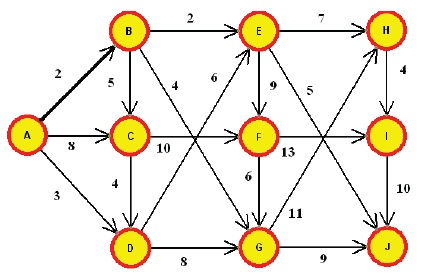
\includegraphics[scale=0.8]{fig/sunario-3/Graf.jpg}%
	\caption{Graf untuk Algoritma Dijkstra}%
	\label{fig:Jalur terpendek}%
\end{center}
\end{figure}

Penyelesaian Figur~\ref{fig:Jalur terpendek} dengan Algoritma Dijkstra ini adalah:
Tentukan bobot dari node yang langsung terhubung dengan node sumber yaitu node A, seperti dari node A ke node B = 2, A ke C = 8, dari A ke D = 3, dan untuk node E,F,G,H,I,J diinisialisasi dengan tanda „-„ karena tidak ada lintasan yang menghubungkan secara langsung dengan node A. kemudian predecessor(node sumber) dari A,B,C,D adalah A, karena jarak dari node tersebut dihitung dari node A, untuk node F,G,H,I,J predecessornya diberi tanda „-„ karena belum ada predecessor yang terhubung langsung dengan node tersebut.

\begin{table}[htbp]
\begin{center}
\begin{tabular}{|c|c|c|c|c|c|c|c|c|c|c|}
\hline
Node & A & B & C & D & E & F & G & H & I & J \\
\hline
Status & 1 & 0 & 0 & 0 & 0 & 0 & 0 & 0 & 0 & 0\\
\hline
Bobot & - & 2 & 8 & 3 & - & - & - & - & - & - \\
\hline
Predecessor & A & A & A & A & - & - & - & - & -  & - \\
\hline
\end{tabular}
\caption{Hasil Iterasi ke-1}
\end{center}
\end{table}

Dari hasil iterasi tabel 1.6 pilih node dengan status „0‟ dan bobot yang paling kecil yaitu B.untuk itu status node B menjadi „1‟ dan predecessornya tetap masih A. jika node B sudah terpilih, maka ada perubahan pada bobot node C,yaitu dari bobot 8 menjadi bobot 7,hal ini terjadi karena bobot 8 didapat dari node A langsung ke node C, padahal ada jalur yang lebih pendek untuk mencapai node C yaitu melewati B, dengan bobot 7, sehingga predecessor pada node C diganti menjadi B, dan karena node B sudah terpilih maka diperoleh node E dengan bobot 4(2+2) dan node G dengan bobot 6(2+4),predecessor node E dan G adalah B. Sehingga diperoleh :

\begin{table}[htbp]
\begin{center}
\begin{tabular}{|c|c|c|c|c|c|c|c|c|c|c|}
\hline
Node & A & B & C & D & E & F & G & H & I & J \\
\hline
Status & 1 & 1 & 0 & 0 & 0 & 0 & 0 & 0 & 0 & 0\\
\hline
Bobot & - & 2 & 7 & 3 & 4 & - & 6 & - & - & - \\
\hline
Predecessor & A & A & B & A & B & - & B & - & -  & - \\
\hline
\end{tabular}
\caption{Hasil Iterasi ke-2}
\end{center}
\end{table}

dapat dilihat dari tabel 1.7 bahwa node D merupakan node dengan bobot paling kecil dibandingkan dengan node-noode sementara yang ada, sehingga status node D sekarang akan berubah menjadi „1‟ dan predecessornya masih tetap A karena jalur terpendek menuju D adalah dari node A. sehingga diperoleh :

\begin{table}[htbp]
\begin{center}
\begin{tabular}{|c|c|c|c|c|c|c|c|c|c|c|}
\hline
Node & A & B & C & D & E & F & G & H & I & J \\
\hline
Status & 1 & 1 & 0 & 1 & 0 & 0 & 0 & 0 & 0 & 0\\
\hline
Bobot & - & 2 & 7 & 3 & 4 & - & 6 & - & - & - \\
\hline
Predecessor & A & A & B & A & B & - & B & - & -  & - \\
\hline
\end{tabular}
\caption{Hasil Iterasi ke-3}
\end{center}
\end{table}

Dari tabel 1.8 selanjutnya didapat bahwa node E memiliki bobot paling kecil, sehingga statusnya berubah menajadi „1‟. Jika node E sudah terpilih, maka node F mempunyai bobot 13, node H=11 dan node j=9 .untuk mencapai node F,H dan J maka harus dari node A kemudian ke node B lalu menuju node E maka predecessor ketiga node tersebut menjadi E. Sehingga diperoleh:

\begin{table}[htbp]
\begin{center}
\begin{tabular}{|c|c|c|c|c|c|c|c|c|c|c|}
\hline
Node & A & B & C & D & E & F & G & H & I & J \\
\hline
Status & 1 & 1 & 0 & 1 & 1 & 0 & 0 & 0 & 0 & 0\\
\hline
Bobot & - & 2 & 7 & 3 & 4 & 13 & 6 & 11 & - & 9 \\
\hline
Predecessor & A & A & B & A & B & E & B & E & -  & E \\
\hline
\end{tabular}
\caption{Hasil Iterasi ke-4}
\end{center}
\end{table}

Kemudian dari tabel 1.9 didapat bahwa node G memiliki bobt paling kecil, sehingga statusnya akan berubah menjadi „1‟, predecessornya masih tetap B. jika node G sudah terpilih maka akan ada perubahan bobot pada node F dari bobot 13 menjadi 12, hal ini terjadi karena setelah dihitung rute terpendek menuju F adalah dari node G kalau dibandingkan dengan rute dari node E maka predecessor node F berubah dari E menjadi G. sehingga diperoleh :

\begin{table}[htbp]
\begin{center}
\begin{tabular}{|c|c|c|c|c|c|c|c|c|c|c|}
\hline
Node & A & B & C & D & E & F & G & H & I & J \\
\hline
Status & 1 & 1 & 0 & 1 & 1 & 0 & 1 & 0 & 0 & 0\\
\hline
Bobot & - & 2 & 7 & 3 & 4 & 12 & 6 & 11 & - & 9 \\
\hline
Predecessor & A & A & B & A & B & G & B & E & -  & E \\
\hline
\end{tabular}
\caption{Hasil Iterasi ke-5}
\end{center}
\end{table}

Dan seterusnya algoritma ini akan terus mengulang semua proses yang ada hingga seluruh node yang berstatus sementara „0‟ diubah menjadi berstatus terpilih „1‟, hal ini dapat dilihat dari tabel dan gambar dibawah ini sampai iterasi ke-10:

\begin{table}[htbp]
\begin{center}
\begin{tabular}{|c|c|c|c|c|c|c|c|c|c|c|}
\hline
Node & A & B & C & D & E & F & G & H & I & J \\
\hline
Status & 1 & 1 & 1 & 1 & 1 & 0 & 1 & 0 & 0 & 0\\
\hline
Bobot & - & 2 & 7 & 3 & 4 & 12 & 6 & 11 & - & 9 \\
\hline
Predecessor & A & A & B & A & B & G & B & E & -  & E \\
\hline
\end{tabular}
\caption{Hasil Iterasi ke-6}
\end{center}
\end{table}

\begin{table}[htbp]
\begin{center}
\begin{tabular}{|c|c|c|c|c|c|c|c|c|c|c|}
\hline
Node & A & B & C & D & E & F & G & H & I & J \\
\hline
Status & 1 & 1 & 1 & 1 & 1 & 0 & 1 & 0 & 0 & 1\\
\hline
Bobot & - & 2 & 7 & 3 & 4 & 12 & 6 & 11 & 19 & 9 \\
\hline
Predecessor & A & A & B & A & B & G & B & E & J  & E \\
\hline
\end{tabular}
\caption{Hasil Iterasi ke-7}
\end{center}
\end{table}


\begin{table}[htbp]
\begin{center}
\begin{tabular}{|c|c|c|c|c|c|c|c|c|c|c|}
\hline
Node & A & B & C & D & E & F & G & H & I & J \\
\hline
Status & 1 & 1 & 0 & 1 & 1 & 0 & 1 & 1 & 0 & 0\\
\hline
Bobot & - & 2 & 7 & 3 & 4 & 12 & 6 & 11 & 15 & 9 \\
\hline
Predecessor & A & A & B & A & B & G & B & E & H  & E \\
\hline
\end{tabular}
\caption{Hasil Iterasi ke-8}
\end{center}
\end{table}

\begin{table}[htbp]
\begin{center}
\begin{tabular}{|c|c|c|c|c|c|c|c|c|c|c|}
\hline
Node & A & B & C & D & E & F & G & H & I & J \\
\hline
Status & 1 & 1 & 1 & 1 & 1 & 1 & 1 & 1 & 0 & 1\\
\hline
Bobot & - & 2 & 7 & 3 & 4 & 12 & 6 & 11 & 15 & 9 \\
\hline
Predecessor & A & A & B & A & B & G & B & E & H  & E \\
\hline
\end{tabular}
\caption{Hasil Iterasi ke-9}
\end{center}
\end{table}

\begin{table}[htbp]
\begin{center}
\begin{tabular}{|c|c|c|c|c|c|c|c|c|c|c|}
\hline
Node & A & B & C & D & E & F & G & H & I & J \\
\hline
Status & 1 & 1 & 1 & 1 & 1 & 1 & 1 & 1 & 1 & 1\\
\hline
Bobot & - & 2 & 7 & 3 & 4 & 12 & 6 & 11 & 15 & 9 \\
\hline
Predecessor & A & A & B & A & B & G & B & E & H  & E \\
\hline
\end{tabular}
\caption{Hasil Iterasi ke-10}
\end{center}
\end{table}

\newpage
\begin{figure}[htbp]
\begin{center}
	
\includegraphics[scale=0.5]{fig/sunario-3/A.jpg}%
	\caption{Node Terpilih Hasil Iterasi 1}%
	\label{fig:Node A}%
\end{center}
\end{figure}


\begin{figure}[htbp]
\begin{center}
	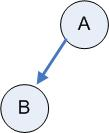
\includegraphics[scale=0.5]{fig/sunario-3/AB.jpg}%
	\caption{Node Terpilih Hasil Iterasi 2}%
\end{center}
\end{figure}


\begin{figure}[htbp]
\begin{center}
	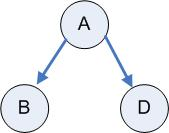
\includegraphics[scale=0.5]{fig/sunario-3/ABD.jpg}%
	\caption{Node Terpilih Hasil Iterasi 3}%
\end{center}
\end{figure}

\begin{figure}[htbp]
\begin{center}
	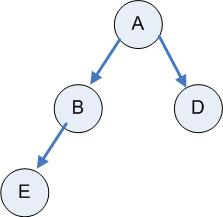
\includegraphics[scale=0.5]{fig/sunario-3/ABDE.jpg}%
	\caption{Node Terpilih Hasil Iterasi 4}%
\end{center}
\end{figure}


\begin{figure}[htbp]
\begin{center}
	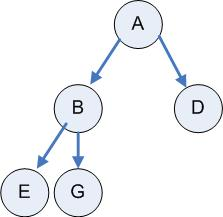
\includegraphics[scale=0.5]{fig/sunario-3/ABDEG.jpg}%
	\caption{Node Terpilih Hasil Iterasi 5}%
\end{center}
\end{figure}

\begin{figure}[htbp]
\begin{center}
	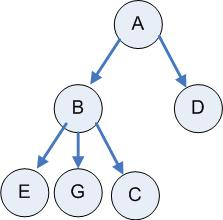
\includegraphics[scale=0.5]{fig/sunario-3/ABDEGC.jpg}%
	\caption{Node Terpilih Hasil Iterasi 6}%
\end{center}
\end{figure}

\begin{figure}[htbp]
\begin{center}
	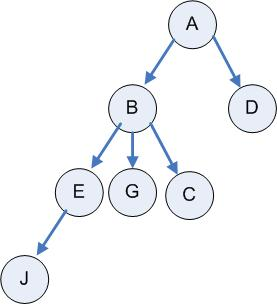
\includegraphics[scale=0.5]{fig/sunario-3/ABDEGCJ.jpg}%
	\caption{Node Terpilih Hasil Iterasi 7}%
\end{center}
\end{figure}

\begin{figure}[htbp]
\begin{center}
	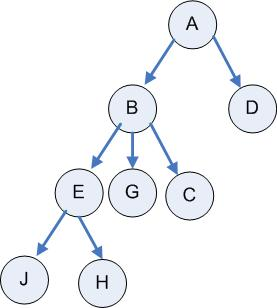
\includegraphics[scale=0.5]{fig/sunario-3/ABDEGCJH.jpg}%
	\caption{Node Terpilih Hasil Iterasi 8}%
\end{center}
\end{figure}


\begin{figure}[htbp]
\begin{center}
	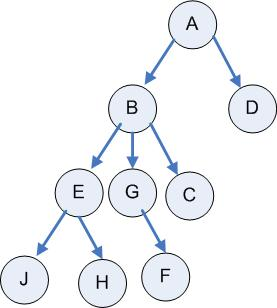
\includegraphics[scale=0.5]{fig/sunario-3/ABDEGCJHF.jpg}%
	\caption{Node Terpilih Hasil Iterasi 9}%
\end{center}
\end{figure}

\begin{figure}[htbp]
\begin{center}
	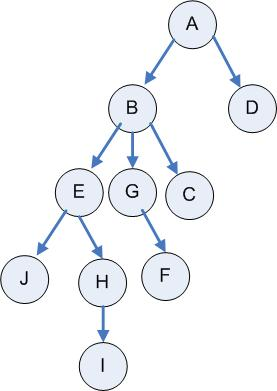
\includegraphics[scale=0.5]{fig/sunario-3/ABDEGCJHFI.jpg}%
	\caption{Node Terpilih Hasil Iterasi 10}%
\end{center}
\end{figure}

\newpage
Setelah mencapai iterasi ke-10 maka semua node yang ada telah berubah status menjadi node terpilih, sehingga akan terbentuk jalur terpendek dari node A ke semua node yang ada, untuk melihat jalur mana yang terpilih dapat ditelusuri dari predecessornya. Itulah yang membedakan algoritma dijkstra dengan algoritma heuristic dimana algoritma dijkstra tidak hanya mencari jalur terpendek dari node awal ke node tujuan tetapi kesemua node yang ada.hal ini dapat dilihat dibawah ini:

$A \triangleright B : A - B : 2 \newline$
$A \triangleright C : A - B - C : 7 \newline$
$A \triangleright D : A - D : 3 \newline$
$A \triangleright E : A - B - E : 4 \newline$
$A \triangleright F : A - B - G - F : 12 \newline$
$A \triangleright G : A - B - G : 6 \newline$
$A \triangleright H : A - B - E - H : 11 \newline$
$A \triangleright I : A - B - E - H - I : 15 \newline$
$A \triangleright J : A - B - E - J : 9 \newline$

Algoritma Dijistrak dalam bahasa phyton dapat dituliskan sebagai berikut :

\lstset{language=Python}
\label{lst:Djistrak}
\begin{lstlisting}[frame=single]
def Dijkstra(G,start,end=None):
 D = {}	# final distances
 P = {}	# predecessors
 Q = priorityDictionary()   #non-final vertex.
 Q[start] = 0
  for v in Q:
  D[v] = Q[v]
  if v == end: 
   break
  for w in G[v]:
  vwLength = D[v] + G[v][w]
  if w in D:
   if vwLength < D[w]:
  	raise ValueError, "Dijkstra: vertex final"   
   elif w not in Q or vwLength < Q[w]:
  	Q[w] = vwLength
  	P[w] = v
		
  return (D,P)
			
def shortestPath(G,start,end):
	D,P = Dijkstra(G,start,end)
	Path = []
	while 1:
		Path.append(end)
		if end == start: break
		end = P[end]
	Path.reverse()
	return Path
\end{lstlisting}

Untuk algoritma Dijkstra, kompleksitas waktu untuk
suatu graf dengan sisi E dan simpul V dapat diekspresikan
dalam bentuk suatu fungsi dari $|E|$ dan $|V|$ sebagai $O(|V^{2}| + |E|) = O(|V^{2}|)$. Dengan sedikit perbaikan, algoritma ini dapat mencapai $O(|E| + |V|) log| =
O(|E| log|V|) ≈ O(|E| + |V| log|V|)$.
\end{enumerate}

\chapter{Teknik \textit{Dynamic Programming}}\label{ch:modul5}

\section{Pengenalan \textit{Dynamic Programming}}
\textit{Dynamic programming} merupakan pendekatan lain dalam memecahkan permasalahan seperti pendekatan \textit{divide and conguer}. Kata \textit{programming} di nama \textit{dynamic programming} tidak berhubungan dengan menulis kode komputer melainkan lebih ke arah metode tabular (kata \textit{dynamic programming} sebenarnya dipopulerkan di bidang matematika bukan ilmu komputer/teknik informatika).

Di \textit{divide and conguer}, permasalahan dipecah menjadi sub-permasalahan yang lebih kecil kemudian dipecahkan secara terpisah dan akhirnya digabungkan. Kelemahan dalam pendekatan ini adalah, beberapa sub-permasalahan sebenarnya memiliki solusi pemecahan yang sama akan tetapi di \textit{divide and conguer} hal itu tidak diperdulikan, melainkan sub-permasalahan yang sama akan diselesaikan berkali-kali sehingga mengakibatkan pemborosan sumber daya komputasional.

Di \textit{dynamic programming} sub-permasalahan yang sama hanya dipecahkan sekali saja dan disimpan solusinya ke dalam tabel (itu sebabnya ia disebut sebagai metode tabular). Apabila ditemukan sub-permasalahan yang sama kelak, maka solusi yang telah disimpan akan dipergunakan kembali.

\textit{Dynamic programming} sering dipakai untuk menyelesaikan permasalahan yang bersifat optimisasi. Permasalahan tersebut mempunyai berbagai macam solusi, akan tetapi hanya ada satu yang nilainya optimal (misalnya nilai paling maksimal atau minimal). Nilai yang paling optimal tersebut disebut juga sebagai solusi optimal dari suatu permasalahan.

Terdapat 4 langkah dalam penyelesaian permasalahan \textit{dynamic programming}:
\begin{enumerate}
	\item Gambarkan struktur dari solusi optimal.
	\item Definisikan nilai dari solusi optimal secara rekursif.
	\item Hitung nilai dari solusi optimal.
	\item Bentuk solusi optimal dari informasi yang sudah dihitung sebelumnya.
\end{enumerate}

\section{Dynamic Programming, Sub-Permasalahan, dan Memoization}

Mari kita mulai penjelasan DP dengan contoh yang paling sederhana terlebih dahulu: perhitungan bilangan fibonacci. Algoritma~\ref{algo:fibonacci-recurse} menunjukkan algoritma perhitungan bilangan fibonacci yang sederhana.

\lstinputlisting[language=Python, 
                 label={algo:fibonacci-recurse},
                 linebackgroundcolor={\ifnum\value{lstnumber}=5\color{codehighlight}\fi},
                 caption=Algoritma Fibonacci Rekursif
                ]
                {code/9-fibonacci.py}

Pada baris ke 5 Algoritma~\ref{algo:fibonacci-recurse} kita dapat melihat bagaimana untuk menyelesaikan perhitungan fibonacci, kita menghitung dua bilangan fibonacci sebelumnya dengan fungsi yang sama (rekursif). Kita dapat menanggap bagian ini sebagai pemecahan masalah ke sub-permasalahan, di mana:

\begin{itemize}
    \item Permasalahan utama kita adalah perhitungan bilangan fibonacci ke $n$, dan
    \item sub-permasalahan adalah menghitung bilangan fibonacci yang lebih kecil ($n - 1$ dan $n - 2$).
\end{itemize}

Kita dapat melihat bagaimana jalur kalkulasi rekursif dari Algoritma~\ref{algo:fibonacci-recurse} pada Gambar~\ref{fig:fibonacci-recurse}.

\begin{figure}
    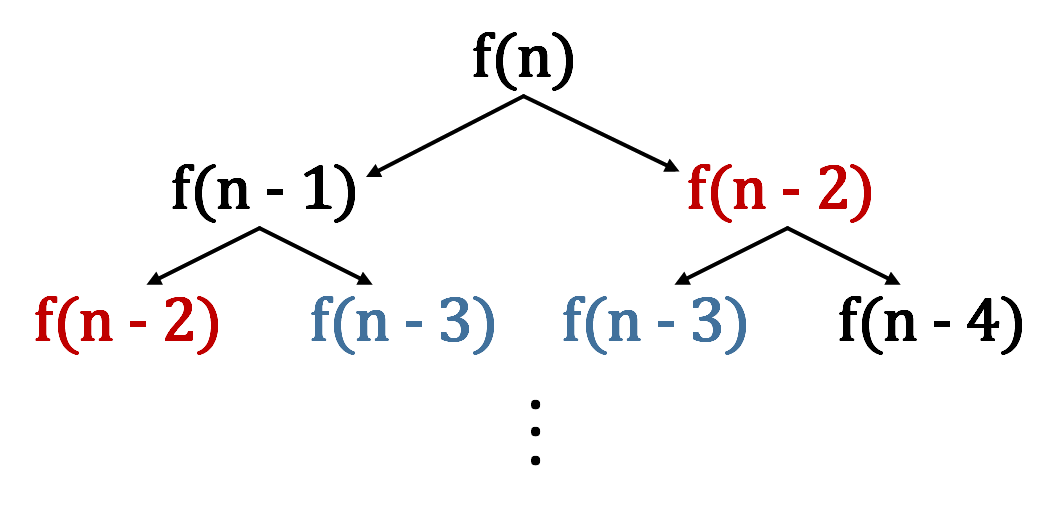
\includegraphics[width=\textwidth,keepaspectratio]{fig/FibonacciCallStack.png}%
	\caption{Proses Pemanggilan Fibonacci}%
	\label{fig:fibonacci-recurse}%
\end{figure}

Pada Gambar~\ref{fig:fibonacci-recurse} kita dapat melihat bagaimana terdapat beberapa fungsi yang perhitungannya kita lakukan beberapa kali, yaitu $f(n - 2)$ dan $f(n - 3)$. Jika perhitungan ini terus diturunkan, kita akan melihat terdapat banyak duplikasi perhitungan seperti ini sampai kita selesai melakukan rekursi. Semakin dalam penurunan fungsi rekursifnya, semakin banyak pula perhitungan kembali yang harus kita lakukan. Karena perhitungan yang dilakukan berulang kali ini, pada dasarnya kita menjalankan $2^n$ langkah pada setiap pemanggilan fungsi fibonacci. Kompleksitas $O(2^n)$ ini tentu saja sangat, sangat buruk.

\marginnote[-4cm]{
    \begin{latihan}
        Bagaimana kita dapat mengetahui bahwa Algoritma~\ref{algo:fibonacci-recurse} memiliki kompleksitas $O(2^n)$? Turunkan perhitungannya!
    \end{latihan}
}

Untuk mengurangi perulangan perhitungan ini, kita dapat menyimpan hasil perhitungan fungsi yang telah kita lakukan sebelumya, seperti yang tampak pada Algoritma~\ref{algo:fibonacci-memoization}.

\lstinputlisting[language=Python, 
                 label={algo:fibonacci-memoization},
                 caption=Algoritma Fibonacci dengan Penyimpanan Hasil,
                 float=t
                ]
                {code/10-fibonacci-memoized.py}

Pada Algoritma~\ref{algo:fibonacci-memoization}, kita dapat melihat bagaimana penyimpanan hasil kalkulasi dilakukan dengan \textit{dictionary}. Pada prakteknya, kita dapat menggunakan struktur data apapun, sesuai dengan kebutuhan kita. Penyimpanan hasil kalkulasi ini akan dapat mengurangi jumlah pemanggilan rekursif yang harus kita lakukan, menjadi seperti pada Gambar~\ref{fig:fibonacci-memoization} saja.

\begin{figure}
    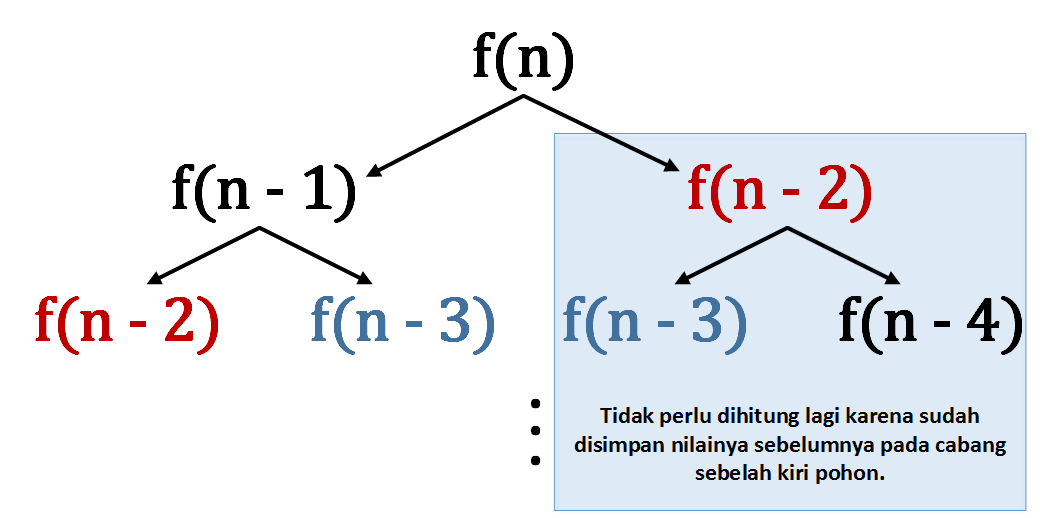
\includegraphics[width=\textwidth,keepaspectratio]{fig/FibonacciDPCallStack.png}%
	\caption{Proses Pemanggilan Fibonacci dengan Penyimpanan Hasil}%
	\label{fig:fibonacci-memoization}%
\end{figure}

Teknik menyimpan hasil kalkulasi agar tidak perlu melakukan perhitungan yang sama berulang kali ini kita kenal dengan nama \textbf{memoization}. Sampai titik ini, kita dapat dikatakan telah menggunakan tekik \textit{dynamic programming} untuk melakukan perhitungan fibonacci. Perhitungan sub-masalah dilakukan secara \textit{lazy} pada Algoritma~\ref{algo:fibonacci-memoization}, karena perhitungan baru dilakukan ketika diperlukan.

Karena banyak sub-masalah yang kita selesaikan melalui memo pada Algoritma~\ref{algo:fibonacci-memoization}, jumlah langkah yang diperlukan untuk menyelesaikan algoritma berkurang menjadi $O(n)$ saja. Kompleksitas $O(1)$ ini didapatkan dengan mengasumsikan pemanggilan isi memori dapat kita anggap sebagai $O(1)$. Pada dasarnya di Algoritma~\ref{algo:fibonacci-memoization} kita melakukan pertukaran jumlah langkah eksekusi dengan memori.

Meskipun telah meningkatkan kompleksitas dengan sangat baik, pada prakteknya Algoritma~\ref{algo:fibonacci-memoization} masih memiliki kekurangan, yaitu penggunaan \textit{stack space} yang terlalu besar. Pada bahasa yang memiliki batasan ukuran stack dan kedalaman rekursif seperti python, hal ini dapat menjadi masalah tersendiri. Untuk menanggulangi hal ini, kita dapat menggunakan pendekatan selain \textit{lazy} pada \textit{dynamic programming}, yaitu pendekatan \textit{bottom-up}.

Algoritma~\ref{algo:fibonacci-bottom-up} menunjukkan cara perhitungan fibonacci secara \textit{bottom-up}.

\lstinputlisting[language=Python, 
                 label={algo:fibonacci-bottom-up},
                 caption=Algoritma Fibonacci Bottom-Up
                ]
                {code/11-fiibonacci-bottom-up.py}

Pada teknik \textit{bottom-up} yang digunakan dalam Algoritma~\ref{algo:fibonacci-bottom-up}, kita terlebih dahulu menentukan urutan operasi yang akan dilakukan. Sebelum mulai melakukan perhitungan, kita mengetahui beberapa hal:

\begin{itemize}
    \item Semua hasil kalkulasi disimpan dalam $memo$.
    \item Pada fibonacci tradisional, kita akan menghitung nilai fibonacci dari $n$ sampai $1$,
    \item bilangan fibonacci selalu membutuhkan dua buah bilangan fibonacci sebelumnya.
    \item Urutan kalkulasi yang dilakukan pada fibonacci tradisional adalah $f(n)$, $f(n - 1)$, $f(n -2)$, dst.
\end{itemize}

Pada pendekatan \textit{bottom-up}, kita hanya semata-mata mengganti urutan operasi dari fibonacci. Karena kita tahu perhitungan fibonacci ke $n$ akan memerlukan perhitungan fibonacci ke $1$ sampai $n$, kita dapat melakukan perhitungan tersebut secara langsung (dari $1$ sampai $n$; kecil ke besar; \textit{bottom-up}) alih-alih menghitung dari $n$ sampai ke $1$ (besar ke kecil; \textit{top-down}) yang apda setiap langkahnya kita harus menunggu hasil perhitungan baru. Perhatikan juga bagaimana inti algoritma (bagian $if n <= 2$) pada Algoritma~\ref{algo:fibonacci-recurse}, ~\ref{algo:fibonacci-memoization}, dan ~\ref{algo:fibonacci-bottom-up} adalah sama. Hal ini menunjukkan bagaimana pada dasarnya kita melakukan perhitungan yang sama, dengan metode yang berbeda dan lebih efisien.

Sampai titik ini kita telah melihat bagian paling mendasar dari \textit{dynamic programming}, yaitu pemecahan sub-masalah dan \textit{memoization}. Bagian lain yang tak kalah pentingnya dari \textit{dynamic programming} adalah optimasi. Mari kita lihat contoh lain yang akan memberikan kita langkah optimasi pada \textit{dynamic programming}.

\section{Optimasi}

Lorem ipsum dolor sit amet

\section{Contoh DP: Pemotongan Rotan}
Sebagai salah satu contoh permasalahan yang bisa diselesaikan dengan menggunakan \textit{dynamic programming}, kita akan menyelesaikan permasalahan pemotongan rotan. 

Sebuah perusahaan membeli berbagai rotan dengan panjang berbeda-beda. Rotan tersebut akan dipotong menjadi beberapa rotan yang lebih pendek kemudian akan dijual lagi. Untuk setiap pemotongan tidak dikenakan biaya. Pihak manajemen dari perusahaan tersebut ingin mengetahui cara paling optimal untuk memotong rotan-rotan tersebut.

Asumsi kita mengetahui untuk setiap nilai $i=1,2,\ldots,$ $p_i$ merupakan harga yang ditetapkan perusahaan tersebut ketika menjual rotan dengan panjang $i$ inci. Panjang dari rotan akan selalu dalam bentuk integer. 

Definisi formal dari permasalahan tersebut adalah sebagai berikut.

\begin{contoh}
\textbf{Permasalahan Pemotongan Rotan}\\
Diketahui sebuah rotan dengan panjang $n$ dan sebuah tabel harga $p_i$ untuk $i=1,2,\ldots,n$, tentukan keuntungan maksimum $r_n$ yang bisa diperoleh dengan memotong rotan menjadi rotan-rotan yang lebih pendek. \\
\textbf{Masukan:}\\
Sebuah \textit{array} $p_i$ dimana $i=1,2,..,n$ dan $p_i$ adalah harga untuk panjang $i$.\\
\textbf{Keluaran:}\\
Sebuah nilai $r_n$ yang merupakan nilai optimal dari pemotongan rotan $n$ dan kemudian dijual. Ada juga kemungkinan rotan tak perlu dipotong tetapi sudah memiliki harga yang tinggi daripada harus dipotong lagi.\\
\end{contoh}

\begin{figure}
\centering
\includegraphics[scale=0.6]{fig/rodCutting.eps}%
\caption{Perbandingan panjang $p_i$ dan harga $i$}%
\label{fig:rodCutting}%
\end{figure}


Sebagai contohnya, ketika $n=4$, sesuai dengan tabel di Gambar \ref{fig:rodCutting} maka jika rotan tidak dipotong ($n=4$) harganya $p_4 = 9$ sedangkan jika dipotong menjadi 2 bagian yang sama panjang ($n=2$) maka harganya menjadi $r_4=p_2+p_2=5+5=10$ yang merupakan nilai optimal (lihat Gambar \ref{fig:rodCutting2}).   

\begin{figure}
\centering
\includegraphics[scale=0.7]{fig/rodCutting2.eps}%
\caption{Berbagai jenis potongan yang mungkin. Potongan yang paling optimal adalah yang bagian (c).}%
\label{fig:rodCutting2}%
\end{figure}

Dengan observasi dan nilai $n$ yang kecil kita bisa menentukan nilai optimal untuk setiap ukuran sebagai berikut. \\
r1 = 1 dari solusi 1 = 1 (tidak potong) ;\\
r2 = 5 dari solusi 2 = 2 (tidak potong) ;\\
r3 = 8 dari solusi 3 = 3 (tidak potong) ;\\
r4 = 10 dari solusi 4 = 2 + 2 ;\\
r5 = 13 dari solusi 5 = 2 + 3 ;\\
r6 = 17 dari solusi 6 = 6 (tidak potong) ;\\
r7 = 18 dari solusi 7 = 1 + 6 or 7 = 2 + 2 + 3 ;\\
r8 = 22 dari solusi 8 = 2 + 6 ;\\
r9 = 25 dari solusi 9 = 3 + 6 ;\\
r10 = 30 dari solusi 10 = 10 (tidak potong).

Banyaknya kemungkinan cara yang ada untuk memotong rotan $n$ adalah $2^{n-1}$ cara yang berbeda. Nilai $2^{n-1}$ didapat melalui perhitungan dimana setiap nilai $i$ sampai $n-1$ (jika panjang $n$ maka ada $n-1$ tempat untuk dipotong) ada 2 kemungkinan yang ada yaitu potong atau tidak potong. Jadi, untuk $n=4$ maka jumlah kemungkinannya adalah $2\times{}2\times{}2 = 8$ atau $2^3$. 

Solusi penyelesaian pemotongan rotan dengan menggunakan algoritma naive rekursif adalah sebagai berikut.

\begin{algorithm}
	\caption{CUT-ROD-NAIVE($p,n$)}
	\label{algo:cutRodNaive}
	\begin{algorithmic}[1]
		\IF{$n == 0$}
			\RETURN 0
		\ENDIF
		\STATE $q=-\infty$
		\FOR{$i$ \TO $n$}
			\STATE $q= max(q, p[i] + $CUT-ROD-NAIVE$(p,n-i))$
		\ENDFOR
	\end{algorithmic}
\end{algorithm}

Sedangkan solusi penyelesaian dengan menggunakan metode \textit{Dynamic Programming} ada dua macam penyelesaian yaitu \textit{Bottom Up} dan \textit{Top Down}.

\begin{algorithm}
	\caption{MEMOIZED-CUT-ROD($p,n$)}
	\label{algo:memoizedCutRod}
	\begin{algorithmic}[1]
		\STATE let $r[0..n]$ be a new array
		\FOR{$i$ \TO $n$}
			\STATE $r[i]=-\infty$
		\ENDFOR
		\RETURN MEMOIZED-CUT-ROD-AUX($p,n,r$)
	\end{algorithmic}
\end{algorithm}

\begin{algorithm}
	\caption{MEMOIZED-CUT-ROD-AUX($p,n,r$)}
	\label{algo:memoizedCutRodAux}
	\begin{algorithmic}[1]
		\IF{$r[n]\geq 0$}
			\RETURN $r[n]$
		\ENDIF
		\IF{$n==0$}
			\STATE $q=0$
		\ELSE
			\STATE $q=-\infty$
			\FOR{$i=1$ \TO $n$}
				\STATE $q=max(q,p[i]+$MEMOIZED-CUT-ROD-AUX$(p,n-1,r))$
			\ENDFOR
		\ENDIF
		\STATE $r[n]=q$
		\RETURN $q$
	\end{algorithmic}
\end{algorithm}

\begin{algorithm}
	\caption{BOTTOM-UP-CUT-ROD($p,n$)}
	\label{algo:bottomUpCutRod}
	\begin{algorithmic}[1]
		\STATE let $r[0..n]$ be a new array
		\STATE $r[0] = 0$
		\FOR{$j=1$ \TO $n$}
			\STATE $q=-\infty$
			\FOR{$i=1$ \TO $j$}
				\STATE $q=max(q,p[i]+r[j-i])$
			\ENDFOR
			\STATE $r[j] = q$
		\ENDFOR
		\RETURN $r[n]$
	\end{algorithmic}
\end{algorithm}

Kita bisa menyempurnakan algoritma \ref{algo:bottomUpCutRod} supaya bisa menampilkan solusi dari setiap panjang optimal dari permasalahan pemotongan rotan dengan algoritma berikut.

\begin{algorithm}
	\caption{EXTENDED-BOTTOM-UP-CUT-ROD($p,n$)}
	\label{algo:extBottomUpCutRod}
	\begin{algorithmic}[1]
		\STATE let $r[0..n]$ be a new array
		\STATE $r[0] = 0$
		\FOR{$j=1$ \TO $n$}
			\STATE $q=-\infty$
			\FOR{$i=1$ \TO $j$}
				\IF{$q<p[i]+r[j-i]$}
					\STATE $q=p[i]+r[j-i]$
					\STATE $s[j]=i$
				\ENDIF
			\ENDFOR
			\STATE $r[j] = q$
		\ENDFOR
		\RETURN $r[n]$
	\end{algorithmic}
\end{algorithm}

\begin{algorithm}
	\caption{PRINT-CUT-ROD-SOLUTION($p,n$)}
	\label{algo:printCutRodSolution}
	\begin{algorithmic}[1]
		\STATE $(r,s)$ = EXTENDED-BOTTOM-UP-CUT-ROD($r,n$)
		\WHILE{$n>0$}
			\STATE print $s[n]$
			\STATE $n = n - s[n]$
		\ENDWHILE
	\end{algorithmic}
\end{algorithm}

\begin{figure}
\centering
\includegraphics[scale=0.5]{fig/CutRodSolution.eps}%
\caption{Solusi dari permasalahan pemotongan rotan.}%
\label{fig:cutRodSolution}%
\end{figure}

\section{Contoh DP: Pengalian Rangkaian Matriks}

Salah satu permasalahan yang sangat umum di \textit{Dynamic Programming} adalah permasalahan pengalian rangkaian matriks. Dalam masalah ini diberikan sebuah rangkaian matriks $\left\langle A_{1},A_{2},\ldots,A_{n} \right\rangle$ yang terdiri dari $n$ matriks dimana akan dicari pengalian paling optimal dari rangkaian matriks.  

Jika seandainya terdapat 4 buah matriks dalam sebuah rangkaian $\left\langle A_{1},A_{2},A_{3},A_{4} \right\rangle$ maka kemungkinan yang terdapat untuk mengalikan matriks tersebut adalah sebagai berikut.


$(A_{1}(A_{2}(A_{3}A_{4})))$,\\
$(A_{1}((A_{2}A_{3})A_{4}))$,\\
$((A_{1}A_{2})(A_{3}A_{4}))$,\\
$((A_{1}(A_{2}A_{3}))A_{4})$,\\
$(((A_{1}A_{2})A_{3})A_{4})$.

Dari kelima kemungkinan cara pengalian diatas, setiap cara akan memiliki biaya pengalian yang berbeda. Untuk menyederhanakan, kita akan menggunakan 3 buah matriks dalam satu rangkaian $\left\langle A_{1},A_{2},A_{3} \right\rangle$ dengan dimensi dari setiap matriks dalam rangkaian tersebut adalah 10 X 100, 100 X 5 dan 5 X 50. 

Semisalnya kita mengalikan sesuai dengan cara $((A_{1}A_{2})A_{3})$ maka biaya yang diperlukan adalah 10.100.5 = 5000 sesuai dengan perkalian skalar untuk menghitung $A_{1}A_{2}$ ditambah 10.5.50 = 2500 untuk mengalikan hasilnya dengan $A_{3}$. Total dari semua adalah 5000+2500 = 7500.

Seandainya kita mengalikan dengan cara $(A_{1}(A_{2}A_{3}))$ maka perhitungan biayanya adalah: pengalian $A_{2}A_{3}$ sebesar 100.5.50 = 25000 ditambah dengan 10.100.50 = 50000 untuk mengalikan hasilnya dengan $A_{1}$. Total biaya adalah 25000+50000 = 75000. Dari dua cara pengalian bisa disimpulkan bahwa pengalian dengan cara pertama lebih efisien.

Berdasarkan illustrasi diatas, maka bisa permasalahan perkalian matriks bisa dituliskan sebagai berikut. Diberikan sebuah rangkaian $\left\langle A_{1},A_{2},\ldots,A_{n} \right\rangle$ dari $n$ matriks dimana $i=1,2,\ldots,n$ dan matriks $A_{i}$ memiliki dimensi $p_{i-1}xp_{i}$, carilah cara pengalian yang memiliki biaya perkalian skalar yang terkecil.

Secara matematis solusi dari permasalahan perkalian matriks bisa ditulis sebagai:

\begin{figure}
	\includegraphics[scale=0.4]{fig/math-matrix.eps}%
	\label{fig:math-matrix}%
\end{figure}

Algoritma yang digunakan untuk mencari solusi optimal dari perkalian matriks adalah sebagai berikut.

\begin{algorithm}
	\caption{MATRIX-CHAIN-ORDER($p$)}
	\label{algo:matrixChainOrder}
	\begin{algorithmic}[1]
		\STATE $n=p.length-1$
		\STATE let $m[1..n,1..n]$ and $s[1..n-1,2..n]$ be new tables
		\FOR{$i=1 $\TO$n$}
			\STATE $m[i,i] = 0$
		\ENDFOR
		\FOR{$l=2$ \TO$n$}
			\FOR{$i=1$ \TO$n-l+1$}
				\STATE $j=i+l-1$
				\STATE $m[i,j]=\infty$
				\FOR{$k=i$ \TO$j-1$}
					\STATE $q=m[i,k]+m[k+1,j]+p_{i-1}p_{k}p_{j}$
					\IF{$q<m[i,j]$}
						\STATE $m[i,j]=q$
						\STATE $s[i,j]=k$
					\ENDIF			
				\ENDFOR
			\ENDFOR
		\ENDFOR
		\RETURN $m$ and $s$
	\end{algorithmic}
\end{algorithm}

Dari Algoritma \ref{algo:matrixChainOrder} akan dihasilkan dua buah matriks yaitu tabel $m$ dan tabel$s$. Sebagai contoh, jika rangkaian matriks yang digunakan adalah sebagai berikut.

\begin{figure}
	\includegraphics[scale=0.5]{fig/matrix.eps}%
	\label{fig:matrix}%
\end{figure}

maka tabel $m$ dan tabel $s$ yang diperoleh adalah:
\begin{figure}
	\includegraphics[scale=0.7]{fig/matrix2.eps}%
	\caption{Tabel $m$ dan $s$ yang diperoleh dengan jumlah matriks sebanyak 6 buah}
	\label{fig:matrix2}%
\end{figure}



\end{document}
